% Options for packages loaded elsewhere
\PassOptionsToPackage{unicode}{hyperref}
\PassOptionsToPackage{hyphens}{url}
%
\documentclass[
]{article}
\usepackage{amsmath,amssymb}
\usepackage{lmodern}
\usepackage{iftex}
\ifPDFTeX
  \usepackage[T1]{fontenc}
  \usepackage[utf8]{inputenc}
  \usepackage{textcomp} % provide euro and other symbols
\else % if luatex or xetex
  \usepackage{unicode-math}
  \defaultfontfeatures{Scale=MatchLowercase}
  \defaultfontfeatures[\rmfamily]{Ligatures=TeX,Scale=1}
\fi
% Use upquote if available, for straight quotes in verbatim environments
\IfFileExists{upquote.sty}{\usepackage{upquote}}{}
\IfFileExists{microtype.sty}{% use microtype if available
  \usepackage[]{microtype}
  \UseMicrotypeSet[protrusion]{basicmath} % disable protrusion for tt fonts
}{}
\makeatletter
\@ifundefined{KOMAClassName}{% if non-KOMA class
  \IfFileExists{parskip.sty}{%
    \usepackage{parskip}
  }{% else
    \setlength{\parindent}{0pt}
    \setlength{\parskip}{6pt plus 2pt minus 1pt}}
}{% if KOMA class
  \KOMAoptions{parskip=half}}
\makeatother
\usepackage{xcolor}
\usepackage[margin=1in]{geometry}
\usepackage{color}
\usepackage{fancyvrb}
\newcommand{\VerbBar}{|}
\newcommand{\VERB}{\Verb[commandchars=\\\{\}]}
\DefineVerbatimEnvironment{Highlighting}{Verbatim}{commandchars=\\\{\}}
% Add ',fontsize=\small' for more characters per line
\usepackage{framed}
\definecolor{shadecolor}{RGB}{248,248,248}
\newenvironment{Shaded}{\begin{snugshade}}{\end{snugshade}}
\newcommand{\AlertTok}[1]{\textcolor[rgb]{0.94,0.16,0.16}{#1}}
\newcommand{\AnnotationTok}[1]{\textcolor[rgb]{0.56,0.35,0.01}{\textbf{\textit{#1}}}}
\newcommand{\AttributeTok}[1]{\textcolor[rgb]{0.77,0.63,0.00}{#1}}
\newcommand{\BaseNTok}[1]{\textcolor[rgb]{0.00,0.00,0.81}{#1}}
\newcommand{\BuiltInTok}[1]{#1}
\newcommand{\CharTok}[1]{\textcolor[rgb]{0.31,0.60,0.02}{#1}}
\newcommand{\CommentTok}[1]{\textcolor[rgb]{0.56,0.35,0.01}{\textit{#1}}}
\newcommand{\CommentVarTok}[1]{\textcolor[rgb]{0.56,0.35,0.01}{\textbf{\textit{#1}}}}
\newcommand{\ConstantTok}[1]{\textcolor[rgb]{0.00,0.00,0.00}{#1}}
\newcommand{\ControlFlowTok}[1]{\textcolor[rgb]{0.13,0.29,0.53}{\textbf{#1}}}
\newcommand{\DataTypeTok}[1]{\textcolor[rgb]{0.13,0.29,0.53}{#1}}
\newcommand{\DecValTok}[1]{\textcolor[rgb]{0.00,0.00,0.81}{#1}}
\newcommand{\DocumentationTok}[1]{\textcolor[rgb]{0.56,0.35,0.01}{\textbf{\textit{#1}}}}
\newcommand{\ErrorTok}[1]{\textcolor[rgb]{0.64,0.00,0.00}{\textbf{#1}}}
\newcommand{\ExtensionTok}[1]{#1}
\newcommand{\FloatTok}[1]{\textcolor[rgb]{0.00,0.00,0.81}{#1}}
\newcommand{\FunctionTok}[1]{\textcolor[rgb]{0.00,0.00,0.00}{#1}}
\newcommand{\ImportTok}[1]{#1}
\newcommand{\InformationTok}[1]{\textcolor[rgb]{0.56,0.35,0.01}{\textbf{\textit{#1}}}}
\newcommand{\KeywordTok}[1]{\textcolor[rgb]{0.13,0.29,0.53}{\textbf{#1}}}
\newcommand{\NormalTok}[1]{#1}
\newcommand{\OperatorTok}[1]{\textcolor[rgb]{0.81,0.36,0.00}{\textbf{#1}}}
\newcommand{\OtherTok}[1]{\textcolor[rgb]{0.56,0.35,0.01}{#1}}
\newcommand{\PreprocessorTok}[1]{\textcolor[rgb]{0.56,0.35,0.01}{\textit{#1}}}
\newcommand{\RegionMarkerTok}[1]{#1}
\newcommand{\SpecialCharTok}[1]{\textcolor[rgb]{0.00,0.00,0.00}{#1}}
\newcommand{\SpecialStringTok}[1]{\textcolor[rgb]{0.31,0.60,0.02}{#1}}
\newcommand{\StringTok}[1]{\textcolor[rgb]{0.31,0.60,0.02}{#1}}
\newcommand{\VariableTok}[1]{\textcolor[rgb]{0.00,0.00,0.00}{#1}}
\newcommand{\VerbatimStringTok}[1]{\textcolor[rgb]{0.31,0.60,0.02}{#1}}
\newcommand{\WarningTok}[1]{\textcolor[rgb]{0.56,0.35,0.01}{\textbf{\textit{#1}}}}
\usepackage{longtable,booktabs,array}
\usepackage{calc} % for calculating minipage widths
% Correct order of tables after \paragraph or \subparagraph
\usepackage{etoolbox}
\makeatletter
\patchcmd\longtable{\par}{\if@noskipsec\mbox{}\fi\par}{}{}
\makeatother
% Allow footnotes in longtable head/foot
\IfFileExists{footnotehyper.sty}{\usepackage{footnotehyper}}{\usepackage{footnote}}
\makesavenoteenv{longtable}
\usepackage{graphicx}
\makeatletter
\def\maxwidth{\ifdim\Gin@nat@width>\linewidth\linewidth\else\Gin@nat@width\fi}
\def\maxheight{\ifdim\Gin@nat@height>\textheight\textheight\else\Gin@nat@height\fi}
\makeatother
% Scale images if necessary, so that they will not overflow the page
% margins by default, and it is still possible to overwrite the defaults
% using explicit options in \includegraphics[width, height, ...]{}
\setkeys{Gin}{width=\maxwidth,height=\maxheight,keepaspectratio}
% Set default figure placement to htbp
\makeatletter
\def\fps@figure{htbp}
\makeatother
\setlength{\emergencystretch}{3em} % prevent overfull lines
\providecommand{\tightlist}{%
  \setlength{\itemsep}{0pt}\setlength{\parskip}{0pt}}
\setcounter{secnumdepth}{-\maxdimen} % remove section numbering
\ifLuaTeX
  \usepackage{selnolig}  % disable illegal ligatures
\fi
\IfFileExists{bookmark.sty}{\usepackage{bookmark}}{\usepackage{hyperref}}
\IfFileExists{xurl.sty}{\usepackage{xurl}}{} % add URL line breaks if available
\urlstyle{same} % disable monospaced font for URLs
\hypersetup{
  pdftitle={Final Project},
  pdfauthor={Lihao Liu, Zikang Chen, Hinn Zhang},
  hidelinks,
  pdfcreator={LaTeX via pandoc}}

\title{Final Project}
\author{Lihao Liu, Zikang Chen, Hinn Zhang}
\date{}

\begin{document}
\maketitle

{
\setcounter{tocdepth}{2}
\tableofcontents
}
\hypertarget{importing-libraries}{%
\subsubsection{Importing libraries}\label{importing-libraries}}

Here we will load all the packages we need for this project.

\begin{Shaded}
\begin{Highlighting}[]
\FunctionTok{library}\NormalTok{(tidyverse)}
\FunctionTok{library}\NormalTok{(dplyr)}
\FunctionTok{library}\NormalTok{(skimr)}
\FunctionTok{library}\NormalTok{(viridis)}
\FunctionTok{library}\NormalTok{(tidymodels)}
\FunctionTok{library}\NormalTok{(ggridges)}
\FunctionTok{library}\NormalTok{(rmdformats)}
\end{Highlighting}
\end{Shaded}

\hypertarget{introduction}{%
\subsection{Introduction}\label{introduction}}

Imagine sitting on your couch and thinking about winding down from a day
of busy work. You turn on your streaming services to pick your movie for
the night. And yet, you are now just realizing that the paradox of
choice reveals the real challenge of the day. Despite having thousands
of movies, TV shows, and video content available at our fingertips, we
often find ourselves scrolling through countless options but still not
being able to decide.

Some might argue that the existing recommendation systems that are based
on prior searching and watch history help elevate the effort of finding
taste-matching content.\footnote{\url{https://towardsdatascience.com/the-4-recommendation-engines-that-can-predict-your-movie-tastes-109dc4e10c52}}
However, this might not hold true for everyone. Research has shown that
history-based algorithms do not account for individual differences, such
as personalities, which largely affect the user's willingness to accept
the recommendations.\footnote{\url{https://link.springer.com/article/10.1007/s10796-017-9800-0}}
Another channel that does not constrain options to within the scope of
users' preference to get inspiration for a movie night is by referring
to online user ratings, such as those on IMDb. Similar to online
shopping, checking out the reviews before committing three hours to a
movie gives reassurance and a chance to quantitatively compare choices.

These voluntary ratings are vital for saving time and getting valuable
insights into a movie's strengths and weaknesses. Yet, how reliable are
the user reviews? Some researchers have found an increasing discrepancy
between critic scores and user ratings.\footnote{\url{https://stephenfollows.com/are-film-critics-becoming-out-of-sync-with-audiences/}}
And that the general public is giving out less indicative scores of the
quality of the film. Besides the uncertainty on credibility, user
reviews progressively suffer from the lack of variability in user
diversity.\footnote{\url{https://news.usc.edu/144379/usc-study-finds-film-critics-like-filmmakers-are-largely-white-and-male/}}
These aforementioned phenomena give rise to the question of whether user
reviews lose their value over time. Consequently, in this project, we
aim to analyze user reviews to offer more context for users to
effectively and correctly interpret online information about movies.

To further investigate movie reviews, we identified the popular movie
review site IMDb as the source of user comments and ratings of movies
available on the most-anticipated streaming service Netflix as the
research scope. Our quantitative analysis considers user scores as the
component to evaluate the underlying trend among user inputs. This
approach is based on the typical user flow. Specifically, users enquire
about the quality of a movie through three steps: search for the movie,
look at the rating scores, and click to see textual reviews if
interested or necessary. User rating scores are the first-available
information in the process and should have a deciding factor in the
selection process.

\hypertarget{problem-statement}{%
\subsection{Problem Statement}\label{problem-statement}}

Moviegoers who are interested in the evaluation of movies before
consumption has limited knowledge about how online user reviews work and
their subjectivity to misinformation. By looking at the trend of recent
year's reviews, we hope to achieve a more guided overview of online
viewer ratings to provide a better decision-making process for viewers.

Alternatively, are the reviews available on IMDb reliable in correctly
reflecting the quality of the movie or are they influenced by external
factors that are less relevant to movies? Therefore, we identify the
following variables related to movies in order to investigate further.

\begin{enumerate}
\def\labelenumi{\arabic{enumi}.}
\tightlist
\item
  Release year: Do people rate movies differently over the years since
  2010?
\item
  Genre: Do movies receive lower/higher ratings due to their genres?
\item
  Holiday season: Does a movie released during a holiday season receive
  a higher/lower rating than a movie released during other times of the
  year?
\end{enumerate}

\hypertarget{data}{%
\subsection{Data}\label{data}}

The two datasets for this project are collected from Kaggle. The first
dataset, ``Netflix Movies And TV Shows'', contains a series of
information, including:

\begin{itemize}
\tightlist
\item
  \texttt{type}: the type of movie and TV shows
\item
  \texttt{title}: title of the show
\item
  \texttt{director}: director of the movie/show
\item
  \texttt{cast}: actors and actresses involved in the movie/show
\item
  \texttt{country}: Country of origin
\item
  \texttt{date\_added}: Date added to Netflix
\item
  \texttt{release\_year}: the release year of the show
\item
  \texttt{rating}: TV rating of the movie/show (eg. PG-13, TV-MA)
\item
  \texttt{duration}: length of the movie/show
\item
  \texttt{listed\_in}: genre
\item
  \texttt{description}: the summary description of the movie/show
\end{itemize}

The second dataset, ``Netflix popular movies dataset'', contains an
extra column of user ratings and votes to complement the first dataset,
including:

\begin{itemize}
\tightlist
\item
  \texttt{rating}: users' ratings on IMDb
\item
  \texttt{votes}: the number of ratings a show/movie receives
\end{itemize}

We plan to merge the two datasets as the second dataset contains ratings
for movies while the first dataset consists of all movies (as opposed to
popular shows in the second dataset).

\hypertarget{data-import}{%
\subsubsection{Data Import}\label{data-import}}

Here we will import the csv file into the studio and take a look at the
data set:

\begin{Shaded}
\begin{Highlighting}[]
\NormalTok{data }\OtherTok{\textless{}{-}} \FunctionTok{read\_csv}\NormalTok{(}\StringTok{"netflix\_titles.csv"}\NormalTok{) }
\end{Highlighting}
\end{Shaded}

\begin{verbatim}
## Rows: 8807 Columns: 12
## -- Column specification --------------------------------------------------------
## Delimiter: ","
## chr (11): show_id, type, title, director, cast, country, date_added, rating,...
## dbl  (1): release_year
## 
## i Use `spec()` to retrieve the full column specification for this data.
## i Specify the column types or set `show_col_types = FALSE` to quiet this message.
\end{verbatim}

\begin{Shaded}
\begin{Highlighting}[]
\NormalTok{movies }\OtherTok{\textless{}{-}} \FunctionTok{read\_csv}\NormalTok{(}\StringTok{"n\_movies.csv"}\NormalTok{)}
\end{Highlighting}
\end{Shaded}

\begin{verbatim}
## Rows: 9957 Columns: 9
## -- Column specification --------------------------------------------------------
## Delimiter: ","
## chr (7): title, year, certificate, duration, genre, description, stars
## dbl (1): rating
## num (1): votes
## 
## i Use `spec()` to retrieve the full column specification for this data.
## i Specify the column types or set `show_col_types = FALSE` to quiet this message.
\end{verbatim}

\begin{Shaded}
\begin{Highlighting}[]
\FunctionTok{glimpse}\NormalTok{(data)}
\end{Highlighting}
\end{Shaded}

\begin{verbatim}
## Rows: 8,807
## Columns: 12
## $ show_id      <chr> "s1", "s2", "s3", "s4", "s5", "s6", "s7", "s8", "s9", "s1~
## $ type         <chr> "Movie", "TV Show", "TV Show", "TV Show", "TV Show", "TV ~
## $ title        <chr> "Dick Johnson Is Dead", "Blood & Water", "Ganglands", "Ja~
## $ director     <chr> "Kirsten Johnson", NA, "Julien Leclercq", NA, NA, "Mike F~
## $ cast         <chr> NA, "Ama Qamata, Khosi Ngema, Gail Mabalane, Thabang Mola~
## $ country      <chr> "United States", "South Africa", NA, NA, "India", NA, NA,~
## $ date_added   <chr> "September 25, 2021", "September 24, 2021", "September 24~
## $ release_year <dbl> 2020, 2021, 2021, 2021, 2021, 2021, 2021, 1993, 2021, 202~
## $ rating       <chr> "PG-13", "TV-MA", "TV-MA", "TV-MA", "TV-MA", "TV-MA", "PG~
## $ duration     <chr> "90 min", "2 Seasons", "1 Season", "1 Season", "2 Seasons~
## $ listed_in    <chr> "Documentaries", "International TV Shows, TV Dramas, TV M~
## $ description  <chr> "As her father nears the end of his life, filmmaker Kirst~
\end{verbatim}

\begin{Shaded}
\begin{Highlighting}[]
\FunctionTok{glimpse}\NormalTok{(movies)}
\end{Highlighting}
\end{Shaded}

\begin{verbatim}
## Rows: 9,957
## Columns: 9
## $ title       <chr> "Cobra Kai", "The Crown", "Better Call Saul", "Devil in Oh~
## $ year        <chr> "(2018– )", "(2016– )", "(2015–2022)", "(2022)", "(2022– )~
## $ certificate <chr> "TV-14", "TV-MA", "TV-MA", "TV-MA", "TV-MA", "TV-MA", "TV-~
## $ duration    <chr> "30 min", "58 min", "46 min", "356 min", "24 min", "45 min~
## $ genre       <chr> "Action, Comedy, Drama", "Biography, Drama, History", "Cri~
## $ rating      <dbl> 8.5, 8.7, 8.9, 5.9, 8.6, 7.8, 9.2, 9.5, 6.3, 6.2, 8.7, 4.7~
## $ description <chr> "Decades after their 1984 All Valley Karate Tournament bou~
## $ stars       <chr> "['Ralph Macchio, ', 'William Zabka, ', 'Courtney Henggele~
## $ votes       <dbl> 177031, 199885, 501384, 9773, 15413, 116358, 502160, 18313~
\end{verbatim}

We see that the original dataset with movie's features contains 8807
observations with 12 variables, and the dataset with movie ratings
contains 9957 observations and 9 variables.

\hypertarget{data-wrangling}{%
\subsubsection{Data Wrangling}\label{data-wrangling}}

Since the data set we eventually wish to utilize is not two separate
tibbles, we need to find a way to extract the useful columns and take
the combination of two data sets and conduct our analysis from the
integrated tibble.

First, we will merge the two data sets so as to get each movie's rating
and votes and also leave only movies with us, since we are not
considering TV shows.

\begin{Shaded}
\begin{Highlighting}[]
\CommentTok{\#filter out only movies}
\NormalTok{data }\OtherTok{\textless{}{-}}\NormalTok{ data }\SpecialCharTok{|\textgreater{}} \FunctionTok{filter}\NormalTok{(type }\SpecialCharTok{==} \StringTok{"Movie"}\NormalTok{)}

\CommentTok{\#get only the rating and voting columns}
\NormalTok{movies }\OtherTok{\textless{}{-}}\NormalTok{ movies[, }\FunctionTok{c}\NormalTok{(}\StringTok{"title"}\NormalTok{, }\StringTok{"rating"}\NormalTok{, }\StringTok{"votes"}\NormalTok{)]}

\CommentTok{\#merge the two data sets}
\NormalTok{merged }\OtherTok{\textless{}{-}} \FunctionTok{merge}\NormalTok{(data, movies, }\AttributeTok{by =} \StringTok{"title"}\NormalTok{)}
\end{Highlighting}
\end{Shaded}

Then we want to rename the columns to make their names consistent.

\begin{Shaded}
\begin{Highlighting}[]
\CommentTok{\# rename columns}
\NormalTok{merged }\OtherTok{\textless{}{-}}\NormalTok{ merged }\SpecialCharTok{|\textgreater{}}
  \FunctionTok{rename}\NormalTok{(}\StringTok{"certificate"} \OtherTok{=} \StringTok{"rating.x"}\NormalTok{,}
         \StringTok{"rating"} \OtherTok{=} \StringTok{"rating.y"}\NormalTok{)}
\end{Highlighting}
\end{Shaded}

We also want to change the format of the date column from character to
date for easier access.

\begin{Shaded}
\begin{Highlighting}[]
\CommentTok{\# convert dates from character to date type}
\NormalTok{merged}\SpecialCharTok{$}\NormalTok{date\_added }\OtherTok{\textless{}{-}} \FunctionTok{mdy}\NormalTok{(merged}\SpecialCharTok{$}\NormalTok{date\_added)}
\end{Highlighting}
\end{Shaded}

Moreover, we extract the month from the date so that we can generate
plots in the EDA section.

\begin{Shaded}
\begin{Highlighting}[]
\CommentTok{\# create a month column}
\NormalTok{merged}\SpecialCharTok{$}\NormalTok{month }\OtherTok{\textless{}{-}} \FunctionTok{month}\NormalTok{(merged}\SpecialCharTok{$}\NormalTok{date\_added)}
\end{Highlighting}
\end{Shaded}

Since we decide to set the unit of durations of movies into minutes, we
can clean the column of Duration into a column of integers.

\begin{Shaded}
\begin{Highlighting}[]
\NormalTok{merged}\SpecialCharTok{$}\NormalTok{duration }\OtherTok{\textless{}{-}} \FunctionTok{substring}\NormalTok{(merged}\SpecialCharTok{$}\NormalTok{duration, }\DecValTok{1}\NormalTok{, }\FunctionTok{nchar}\NormalTok{(merged}\SpecialCharTok{$}\NormalTok{duration)}\SpecialCharTok{{-}}\DecValTok{4}\NormalTok{)}
\NormalTok{merged}\SpecialCharTok{$}\NormalTok{duration }\OtherTok{\textless{}{-}} \FunctionTok{as.integer}\NormalTok{(merged}\SpecialCharTok{$}\NormalTok{duration)}
\end{Highlighting}
\end{Shaded}

Let's take a look at the wrangled data set.

\begin{Shaded}
\begin{Highlighting}[]
\FunctionTok{skim}\NormalTok{(merged)}
\end{Highlighting}
\end{Shaded}

\begin{longtable}[]{@{}ll@{}}
\caption{Data summary}\tabularnewline
\toprule()
\endhead
Name & merged \\
Number of rows & 1782 \\
Number of columns & 15 \\
\_\_\_\_\_\_\_\_\_\_\_\_\_\_\_\_\_\_\_\_\_\_\_ & \\
Column type frequency: & \\
character & 9 \\
Date & 1 \\
numeric & 5 \\
\_\_\_\_\_\_\_\_\_\_\_\_\_\_\_\_\_\_\_\_\_\_\_\_ & \\
Group variables & None \\
\bottomrule()
\end{longtable}

\textbf{Variable type: character}

\begin{longtable}[]{@{}
  >{\raggedright\arraybackslash}p{(\columnwidth - 14\tabcolsep) * \real{0.1944}}
  >{\raggedleft\arraybackslash}p{(\columnwidth - 14\tabcolsep) * \real{0.1389}}
  >{\raggedleft\arraybackslash}p{(\columnwidth - 14\tabcolsep) * \real{0.1944}}
  >{\raggedleft\arraybackslash}p{(\columnwidth - 14\tabcolsep) * \real{0.0556}}
  >{\raggedleft\arraybackslash}p{(\columnwidth - 14\tabcolsep) * \real{0.0556}}
  >{\raggedleft\arraybackslash}p{(\columnwidth - 14\tabcolsep) * \real{0.0833}}
  >{\raggedleft\arraybackslash}p{(\columnwidth - 14\tabcolsep) * \real{0.1250}}
  >{\raggedleft\arraybackslash}p{(\columnwidth - 14\tabcolsep) * \real{0.1528}}@{}}
\toprule()
\begin{minipage}[b]{\linewidth}\raggedright
skim\_variable
\end{minipage} & \begin{minipage}[b]{\linewidth}\raggedleft
n\_missing
\end{minipage} & \begin{minipage}[b]{\linewidth}\raggedleft
complete\_rate
\end{minipage} & \begin{minipage}[b]{\linewidth}\raggedleft
min
\end{minipage} & \begin{minipage}[b]{\linewidth}\raggedleft
max
\end{minipage} & \begin{minipage}[b]{\linewidth}\raggedleft
empty
\end{minipage} & \begin{minipage}[b]{\linewidth}\raggedleft
n\_unique
\end{minipage} & \begin{minipage}[b]{\linewidth}\raggedleft
whitespace
\end{minipage} \\
\midrule()
\endhead
title & 0 & 1.00 & 2 & 83 & 0 & 1740 & 0 \\
show\_id & 0 & 1.00 & 2 & 5 & 0 & 1740 & 0 \\
type & 0 & 1.00 & 5 & 5 & 0 & 1 & 0 \\
director & 53 & 0.97 & 2 & 167 & 0 & 1461 & 0 \\
cast & 170 & 0.90 & 4 & 575 & 0 & 1512 & 0 \\
country & 105 & 0.94 & 4 & 83 & 0 & 257 & 0 \\
certificate & 0 & 1.00 & 1 & 6 & 0 & 13 & 0 \\
listed\_in & 0 & 1.00 & 6 & 64 & 0 & 171 & 0 \\
description & 0 & 1.00 & 90 & 222 & 0 & 1740 & 0 \\
\bottomrule()
\end{longtable}

\textbf{Variable type: Date}

\begin{longtable}[]{@{}
  >{\raggedright\arraybackslash}p{(\columnwidth - 12\tabcolsep) * \real{0.1750}}
  >{\raggedleft\arraybackslash}p{(\columnwidth - 12\tabcolsep) * \real{0.1250}}
  >{\raggedleft\arraybackslash}p{(\columnwidth - 12\tabcolsep) * \real{0.1750}}
  >{\raggedright\arraybackslash}p{(\columnwidth - 12\tabcolsep) * \real{0.1375}}
  >{\raggedright\arraybackslash}p{(\columnwidth - 12\tabcolsep) * \real{0.1375}}
  >{\raggedright\arraybackslash}p{(\columnwidth - 12\tabcolsep) * \real{0.1375}}
  >{\raggedleft\arraybackslash}p{(\columnwidth - 12\tabcolsep) * \real{0.1125}}@{}}
\toprule()
\begin{minipage}[b]{\linewidth}\raggedright
skim\_variable
\end{minipage} & \begin{minipage}[b]{\linewidth}\raggedleft
n\_missing
\end{minipage} & \begin{minipage}[b]{\linewidth}\raggedleft
complete\_rate
\end{minipage} & \begin{minipage}[b]{\linewidth}\raggedright
min
\end{minipage} & \begin{minipage}[b]{\linewidth}\raggedright
max
\end{minipage} & \begin{minipage}[b]{\linewidth}\raggedright
median
\end{minipage} & \begin{minipage}[b]{\linewidth}\raggedleft
n\_unique
\end{minipage} \\
\midrule()
\endhead
date\_added & 0 & 1 & 2009-11-18 & 2021-09-25 & 2019-06-18 & 921 \\
\bottomrule()
\end{longtable}

\textbf{Variable type: numeric}

\begin{longtable}[]{@{}
  >{\raggedright\arraybackslash}p{(\columnwidth - 20\tabcolsep) * \real{0.1414}}
  >{\raggedleft\arraybackslash}p{(\columnwidth - 20\tabcolsep) * \real{0.1010}}
  >{\raggedleft\arraybackslash}p{(\columnwidth - 20\tabcolsep) * \real{0.1414}}
  >{\raggedleft\arraybackslash}p{(\columnwidth - 20\tabcolsep) * \real{0.0909}}
  >{\raggedleft\arraybackslash}p{(\columnwidth - 20\tabcolsep) * \real{0.0909}}
  >{\raggedleft\arraybackslash}p{(\columnwidth - 20\tabcolsep) * \real{0.0505}}
  >{\raggedleft\arraybackslash}p{(\columnwidth - 20\tabcolsep) * \real{0.0808}}
  >{\raggedleft\arraybackslash}p{(\columnwidth - 20\tabcolsep) * \real{0.0707}}
  >{\raggedleft\arraybackslash}p{(\columnwidth - 20\tabcolsep) * \real{0.0909}}
  >{\raggedleft\arraybackslash}p{(\columnwidth - 20\tabcolsep) * \real{0.0808}}
  >{\raggedright\arraybackslash}p{(\columnwidth - 20\tabcolsep) * \real{0.0606}}@{}}
\toprule()
\begin{minipage}[b]{\linewidth}\raggedright
skim\_variable
\end{minipage} & \begin{minipage}[b]{\linewidth}\raggedleft
n\_missing
\end{minipage} & \begin{minipage}[b]{\linewidth}\raggedleft
complete\_rate
\end{minipage} & \begin{minipage}[b]{\linewidth}\raggedleft
mean
\end{minipage} & \begin{minipage}[b]{\linewidth}\raggedleft
sd
\end{minipage} & \begin{minipage}[b]{\linewidth}\raggedleft
p0
\end{minipage} & \begin{minipage}[b]{\linewidth}\raggedleft
p25
\end{minipage} & \begin{minipage}[b]{\linewidth}\raggedleft
p50
\end{minipage} & \begin{minipage}[b]{\linewidth}\raggedleft
p75
\end{minipage} & \begin{minipage}[b]{\linewidth}\raggedleft
p100
\end{minipage} & \begin{minipage}[b]{\linewidth}\raggedright
hist
\end{minipage} \\
\midrule()
\endhead
release\_year & 0 & 1.00 & 2016.90 & 6.01 & 1944 & 2016.00 & 2018.0 &
2020.00 & 2021 & ▁▁▁▁▇ \\
duration & 1 & 1.00 & 94.94 & 26.93 & 3 & 83.00 & 96.0 & 109.00 & 312 &
▁▇▁▁▁ \\
rating & 20 & 0.99 & 6.19 & 1.10 & 2 & 5.50 & 6.3 & 7.00 & 9 & ▁▂▅▇▁ \\
votes & 20 & 0.99 & 21558.62 & 89565.78 & 8 & 830.25 & 2741.0 & 10761.25
& 1819157 & ▇▁▁▁▁ \\
month & 0 & 1.00 & 6.62 & 3.40 & 1 & 4.00 & 7.0 & 10.00 & 12 & ▇▅▆▆▇ \\
\bottomrule()
\end{longtable}

After data cleaning, the new dataset contains 1782 samples (movies) and
some missing values in columns including ``director'', ``cast'', and
``country''. However, we do not plan to use these features in subsequent
steps.

\begin{Shaded}
\begin{Highlighting}[]
\NormalTok{merged }\SpecialCharTok{|\textgreater{}}
  \FunctionTok{group\_by}\NormalTok{(title) }\SpecialCharTok{|\textgreater{}}
  \FunctionTok{filter}\NormalTok{(}\FunctionTok{n}\NormalTok{() }\SpecialCharTok{\textgreater{}} \DecValTok{1}\NormalTok{)}
\end{Highlighting}
\end{Shaded}

\begin{verbatim}
## # A tibble: 71 x 15
## # Groups:   title [29]
##    title       show_id type  director     cast   country date_added release_year
##    <chr>       <chr>   <chr> <chr>        <chr>  <chr>   <date>            <dbl>
##  1 Aurora      s2844   Movie Cristi Puiu  Crist~ Romani~ 2020-03-04         2010
##  2 Aurora      s2844   Movie Cristi Puiu  Crist~ Romani~ 2020-03-04         2010
##  3 Awake       s747    Movie Mark Raso    Gina ~ United~ 2021-06-09         2021
##  4 Awake       s747    Movie Mark Raso    Gina ~ United~ 2021-06-09         2021
##  5 Blockbuster s6335   Movie July Hygreck Syrus~ France  2018-01-24         2017
##  6 Blockbuster s6335   Movie July Hygreck Syrus~ France  2018-01-24         2017
##  7 Bodyguard   s1675   Movie Siddique     Salma~ India   2020-11-19         2011
##  8 Bodyguard   s1675   Movie Siddique     Salma~ India   2020-11-19         2011
##  9 Death Note  s5319   Movie Adam Wingard Wille~ United~ 2017-08-25         2017
## 10 Death Note  s5319   Movie Adam Wingard Wille~ United~ 2017-08-25         2017
## # i 61 more rows
## # i 7 more variables: certificate <chr>, duration <int>, listed_in <chr>,
## #   description <chr>, rating <dbl>, votes <dbl>, month <dbl>
\end{verbatim}

We observed around 40 possible duplicates in the dataset. Yet, most
repeated entries are re-entries due to missing values or that they are
different movies with the same name (with different ratings). This issue
will be addressed in the analysis automatically.

\hypertarget{analysis}{%
\subsection{Analysis}\label{analysis}}

\hypertarget{exploratory-data-analysis}{%
\subsubsection{Exploratory Data
Analysis}\label{exploratory-data-analysis}}

\hypertarget{how-many-movies-are-released-in-each-year-upto-2021}{%
\paragraph{How many movies are released in each year upto
2021?}\label{how-many-movies-are-released-in-each-year-upto-2021}}

We first want to see when the movies are released in this dataset.

\begin{Shaded}
\begin{Highlighting}[]
\NormalTok{merged }\SpecialCharTok{|\textgreater{}}
  \FunctionTok{ggplot}\NormalTok{(}\FunctionTok{aes}\NormalTok{(}\AttributeTok{x =}\NormalTok{ release\_year)) }\SpecialCharTok{+}
  \FunctionTok{geom\_bar}\NormalTok{(}\AttributeTok{fill =} \StringTok{"\#85B9CC"}\NormalTok{) }\SpecialCharTok{+}
  \FunctionTok{labs}\NormalTok{(}\AttributeTok{x =} \StringTok{"Year released"}\NormalTok{,}
       \AttributeTok{y =} \StringTok{"Number of movies"}\NormalTok{,}
       \AttributeTok{title =} \StringTok{"The number of movies released each year"}\NormalTok{,}
       \AttributeTok{subtitle =} \StringTok{"Most movies are released after 2010"}\NormalTok{) }\SpecialCharTok{+}
  \FunctionTok{theme}\NormalTok{(}\AttributeTok{text =} \FunctionTok{element\_text}\NormalTok{(}\AttributeTok{size =} \DecValTok{15}\NormalTok{),}
        \AttributeTok{plot.title.position =} \StringTok{"plot"}\NormalTok{) }\SpecialCharTok{+}
  \FunctionTok{theme\_minimal}\NormalTok{() }\SpecialCharTok{+}
  \FunctionTok{geom\_vline}\NormalTok{(}\AttributeTok{xintercept =} \DecValTok{2010}\NormalTok{, }\AttributeTok{color =} \StringTok{"black"}\NormalTok{) }\SpecialCharTok{+}
  \FunctionTok{annotate}\NormalTok{(}\StringTok{"text"}\NormalTok{, }\AttributeTok{x =} \DecValTok{2006}\NormalTok{, }\AttributeTok{y =} \DecValTok{300}\NormalTok{, }\AttributeTok{label =} \StringTok{"2010"}\NormalTok{, }\AttributeTok{color =} \StringTok{"black"}\NormalTok{, }\AttributeTok{size =} \DecValTok{4}\NormalTok{) }\SpecialCharTok{+}
  \FunctionTok{theme\_classic}\NormalTok{() }\SpecialCharTok{+}
  \FunctionTok{theme}\NormalTok{(}\AttributeTok{axis.title.x =} \FunctionTok{element\_blank}\NormalTok{(),}
        \AttributeTok{plot.title.position =} \StringTok{"plot"}\NormalTok{,}
        \AttributeTok{axis.text.x =} \FunctionTok{element\_text}\NormalTok{(}\AttributeTok{size =} \FloatTok{7.5}\NormalTok{),}
        \AttributeTok{legend.position =} \StringTok{"none"}\NormalTok{)}
\end{Highlighting}
\end{Shaded}

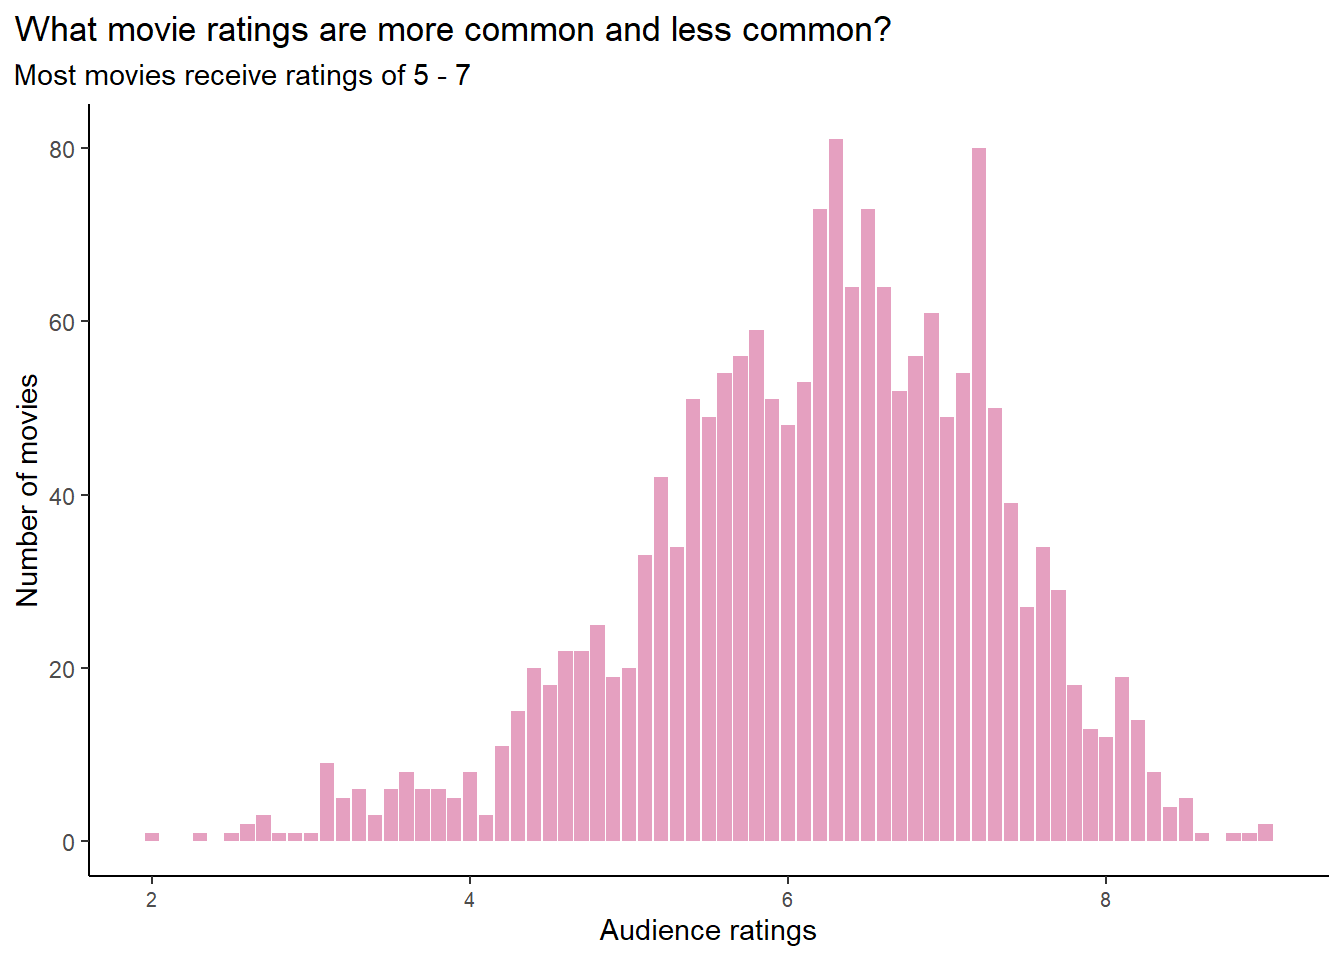
\includegraphics{Final_Project_files/figure-latex/unnamed-chunk-11-1.pdf}

We see that most movies are released after 2010, which suggest most
movies are contemporary. We decide to focus on the movies released after
2010 when we answer our questions in the Data Analysis section, so that
we can safely draw conclusions using our current knowledge.

\hypertarget{the-distribution-of-ratings}{%
\paragraph{The distribution of
ratings}\label{the-distribution-of-ratings}}

We also want to see what ratings do movies generally receive.

\begin{Shaded}
\begin{Highlighting}[]
\NormalTok{merged }\SpecialCharTok{|\textgreater{}}
  \FunctionTok{ggplot}\NormalTok{(}\FunctionTok{aes}\NormalTok{(}\AttributeTok{x =}\NormalTok{ rating)) }\SpecialCharTok{+}
  \FunctionTok{geom\_bar}\NormalTok{(}\AttributeTok{fill =} \StringTok{"\#E5A0C0"}\NormalTok{) }\SpecialCharTok{+}
  \FunctionTok{labs}\NormalTok{(}\AttributeTok{x =} \StringTok{"Audience ratings"}\NormalTok{,}
       \AttributeTok{y =} \StringTok{"Number of movies"}\NormalTok{,}
       \AttributeTok{title =} \StringTok{"What movie ratings are more common and less common?"}\NormalTok{,}
       \AttributeTok{subtitle =} \StringTok{"Most movies receive ratings of 5 {-} 7"}\NormalTok{) }\SpecialCharTok{+}
  \FunctionTok{theme\_classic}\NormalTok{() }\SpecialCharTok{+}
  \FunctionTok{theme}\NormalTok{(}
        \AttributeTok{plot.title.position =} \StringTok{"plot"}\NormalTok{,}
        \AttributeTok{axis.text.x =} \FunctionTok{element\_text}\NormalTok{(}\AttributeTok{size =} \FloatTok{7.5}\NormalTok{),}
        \AttributeTok{legend.position =} \StringTok{"none"}\NormalTok{)}
\end{Highlighting}
\end{Shaded}

\begin{verbatim}
## Warning: Removed 20 rows containing non-finite values (`stat_count()`).
\end{verbatim}

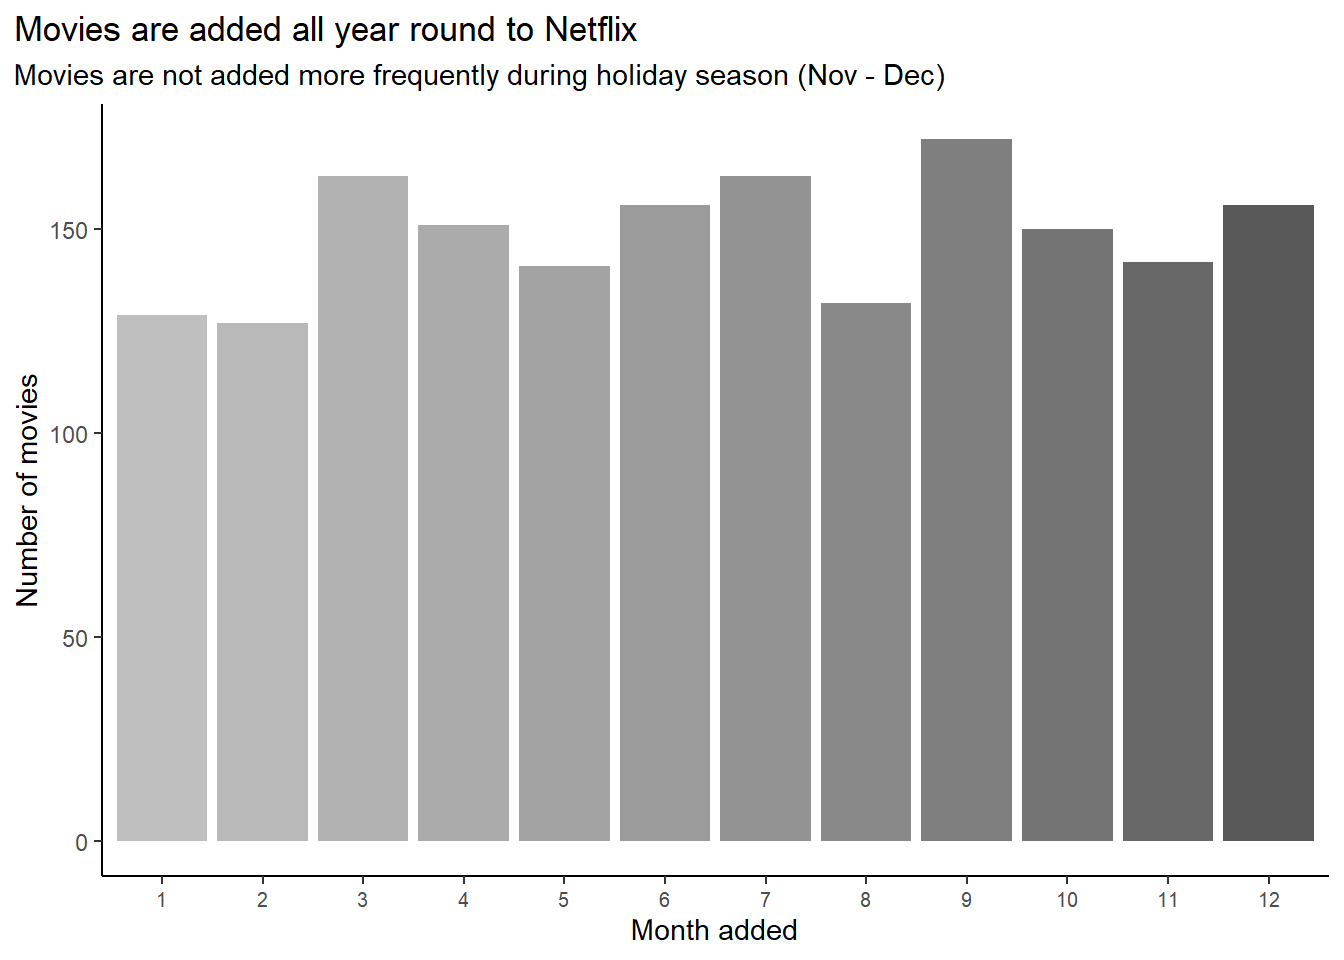
\includegraphics{Final_Project_files/figure-latex/unnamed-chunk-12-1.pdf}

\hypertarget{release-date-of-movies}{%
\paragraph{Release date of movies}\label{release-date-of-movies}}

The plot shows most movies receive a rating in the range of 5 to 7, so
we can infer that a rating above 7 tends to be a high rating, while a
rating below 5 tends to be a low rating.

We also want to see when movies are added to Netflix in a year.

\begin{Shaded}
\begin{Highlighting}[]
\NormalTok{merged }\SpecialCharTok{|\textgreater{}}
  \FunctionTok{ggplot}\NormalTok{(}\FunctionTok{aes}\NormalTok{(}\AttributeTok{x =} \FunctionTok{as.factor}\NormalTok{(month), }\AttributeTok{fill =} \FunctionTok{as.factor}\NormalTok{(month))) }\SpecialCharTok{+}
  \FunctionTok{geom\_bar}\NormalTok{() }\SpecialCharTok{+}
  \FunctionTok{labs}\NormalTok{(}\AttributeTok{x =} \StringTok{"Month added"}\NormalTok{,}
       \AttributeTok{y =} \StringTok{"Number of movies"}\NormalTok{,}
       \AttributeTok{title =} \StringTok{"Movies are added all year round to Netflix"}\NormalTok{,}
       \AttributeTok{subtitle =} \StringTok{"Movies are not added more frequently during holiday season (Nov {-} Dec)"}\NormalTok{) }\SpecialCharTok{+}
  \FunctionTok{scale\_fill\_grey}\NormalTok{(}\AttributeTok{start =} \FloatTok{0.75}\NormalTok{, }\AttributeTok{end =} \FloatTok{0.35}\NormalTok{) }\SpecialCharTok{+}
  \FunctionTok{theme\_classic}\NormalTok{() }\SpecialCharTok{+}
  \FunctionTok{theme}\NormalTok{(}\AttributeTok{legend.position =} \StringTok{"none"}\NormalTok{,}
        \AttributeTok{plot.title.position =} \StringTok{"plot"}\NormalTok{,}
        \AttributeTok{axis.text.x =} \FunctionTok{element\_text}\NormalTok{(}\AttributeTok{size =} \FloatTok{7.5}\NormalTok{))}
\end{Highlighting}
\end{Shaded}

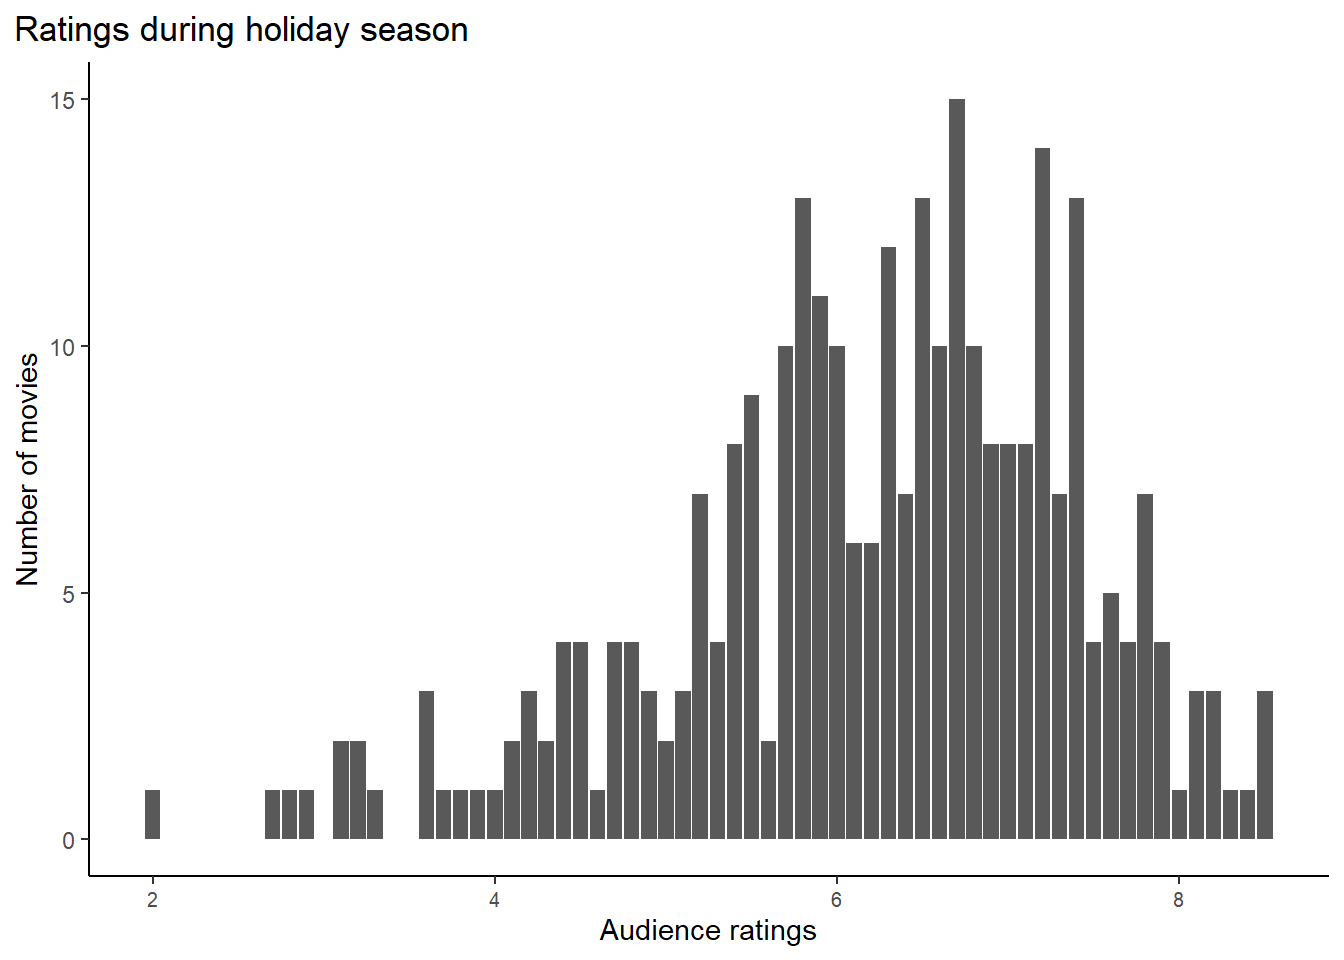
\includegraphics{Final_Project_files/figure-latex/unnamed-chunk-13-1.pdf}

The sample sizes of movies on Netflix are roughly even across all
months, so we can safely compare holiday season movies to non-holiday
season movies.

\hypertarget{how-do-user-ratings-differ-in-different-time-of-the-year}{%
\paragraph{How do user ratings differ in different time of the
year?}\label{how-do-user-ratings-differ-in-different-time-of-the-year}}

\begin{Shaded}
\begin{Highlighting}[]
\NormalTok{merged }\SpecialCharTok{|\textgreater{}}
  \FunctionTok{filter}\NormalTok{(month }\SpecialCharTok{==} \DecValTok{11} \SpecialCharTok{|}\NormalTok{ month }\SpecialCharTok{==} \DecValTok{12}\NormalTok{) }\SpecialCharTok{|\textgreater{}}
  \FunctionTok{ggplot}\NormalTok{(}\FunctionTok{aes}\NormalTok{(}\AttributeTok{x =}\NormalTok{ rating)) }\SpecialCharTok{+}
  \FunctionTok{geom\_bar}\NormalTok{() }\SpecialCharTok{+}
  \FunctionTok{labs}\NormalTok{(}\AttributeTok{x =} \StringTok{"Audience ratings"}\NormalTok{,}
       \AttributeTok{y =} \StringTok{"Number of movies"}\NormalTok{,}
       \AttributeTok{title =} \StringTok{"Ratings during holiday season"}\NormalTok{) }\SpecialCharTok{+}
  \FunctionTok{theme}\NormalTok{(}\AttributeTok{text =} \FunctionTok{element\_text}\NormalTok{(}\AttributeTok{size =} \DecValTok{15}\NormalTok{),}
        \AttributeTok{plot.title.position =} \StringTok{"plot"}\NormalTok{) }\SpecialCharTok{+}
  \FunctionTok{theme\_classic}\NormalTok{() }\SpecialCharTok{+}
  \FunctionTok{theme}\NormalTok{(}
        \AttributeTok{plot.title.position =} \StringTok{"plot"}\NormalTok{,}
        \AttributeTok{axis.text.x =} \FunctionTok{element\_text}\NormalTok{(}\AttributeTok{size =} \FloatTok{7.5}\NormalTok{),}
        \AttributeTok{legend.position =} \StringTok{"none"}\NormalTok{)}
\end{Highlighting}
\end{Shaded}

\begin{verbatim}
## Warning: Removed 3 rows containing non-finite values (`stat_count()`).
\end{verbatim}

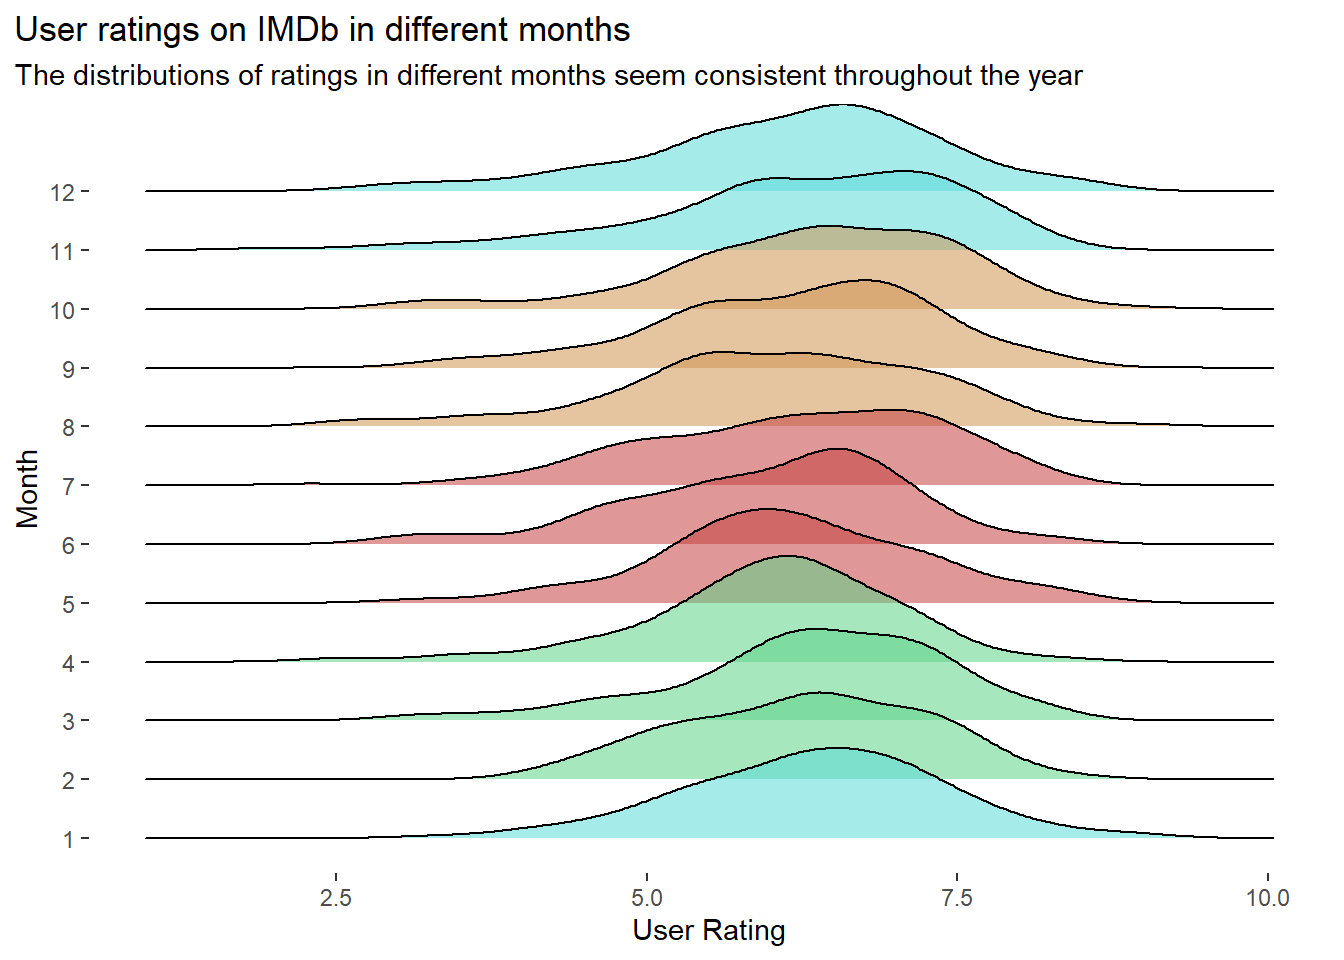
\includegraphics{Final_Project_files/figure-latex/unnamed-chunk-14-1.pdf}

The shape of the distribution of ratings for movies released in the
holiday season is roughly the same as that of all movie ratings. Yet, we
look to investigate the distributions more closely.

\begin{Shaded}
\begin{Highlighting}[]
\NormalTok{merged }\SpecialCharTok{|\textgreater{}}
  \FunctionTok{ggplot}\NormalTok{(}\FunctionTok{aes}\NormalTok{(}\AttributeTok{x =}\NormalTok{ rating, }\AttributeTok{y =} \FunctionTok{as.factor}\NormalTok{(month), }\AttributeTok{fill =} \FunctionTok{as.factor}\NormalTok{(month),}\AttributeTok{alpha =} \FloatTok{0.9}\NormalTok{)) }\SpecialCharTok{+}
  \FunctionTok{geom\_density\_ridges}\NormalTok{() }\SpecialCharTok{+}
  \FunctionTok{labs}\NormalTok{(}\AttributeTok{title =} \StringTok{"User ratings on IMDb in different months"}\NormalTok{,}
       \AttributeTok{subtitle =} \StringTok{"The distributions of ratings in different months seem consistent throughout the year"}\NormalTok{,}
       \AttributeTok{x =} \StringTok{"User Rating"}\NormalTok{,}
       \AttributeTok{y =} \StringTok{"Month"}\NormalTok{) }\SpecialCharTok{+} 
   \FunctionTok{scale\_fill\_manual}\NormalTok{(}\AttributeTok{values =} \FunctionTok{c}\NormalTok{(}\StringTok{"\#5ADAD9"}\NormalTok{,}\StringTok{"\#5ED389"}\NormalTok{,}\StringTok{"\#5ED389"}\NormalTok{,}\StringTok{"\#5ED389"}\NormalTok{,}
                                \StringTok{"\#C44242"}\NormalTok{,}\StringTok{"\#C44242"}\NormalTok{,}\StringTok{"\#C44242"}\NormalTok{,}\StringTok{"\#D09452"}\NormalTok{,}
                                \StringTok{"\#D09452"}\NormalTok{,}\StringTok{"\#D09452"}\NormalTok{,}\StringTok{"\#5ADAD9"}\NormalTok{,}\StringTok{"\#5ADAD9"}\NormalTok{)) }\SpecialCharTok{+} 
  \FunctionTok{theme}\NormalTok{(}\AttributeTok{legend.position =} \StringTok{"none"}\NormalTok{,}
        \AttributeTok{plot.title.position =} \StringTok{"plot"}\NormalTok{,}
        \AttributeTok{panel.grid.major.x =} \FunctionTok{element\_blank}\NormalTok{(),}
        \AttributeTok{panel.grid.minor.x =} \FunctionTok{element\_blank}\NormalTok{(),}
        \AttributeTok{panel.grid.major.y =} \FunctionTok{element\_blank}\NormalTok{(),}
        \AttributeTok{panel.grid.minor.y =} \FunctionTok{element\_blank}\NormalTok{(),}
        \AttributeTok{panel.background =} \FunctionTok{element\_blank}\NormalTok{())}
\end{Highlighting}
\end{Shaded}

\begin{verbatim}
## Picking joint bandwidth of 0.345
\end{verbatim}

\begin{verbatim}
## Warning: Removed 20 rows containing non-finite values
## (`stat_density_ridges()`).
\end{verbatim}

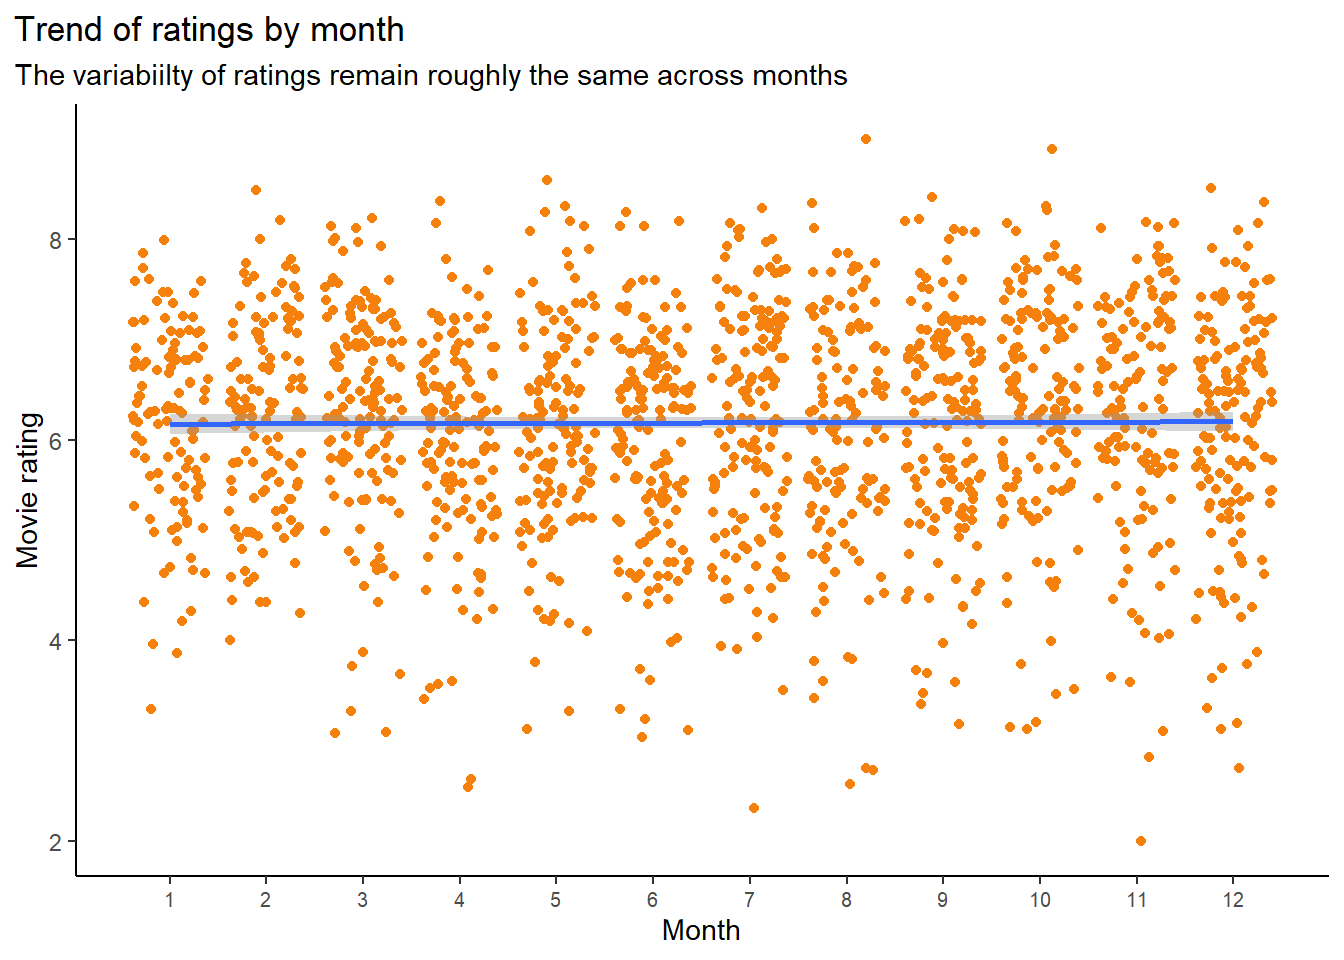
\includegraphics{Final_Project_files/figure-latex/unnamed-chunk-15-1.pdf}

The above visualization contains distribution of user ratings during all
12 months during a year. No significant seasonal bias is observed in
terms of scores of movies.

\begin{Shaded}
\begin{Highlighting}[]
\NormalTok{merged }\SpecialCharTok{|\textgreater{}}
  \FunctionTok{filter}\NormalTok{(release\_year }\SpecialCharTok{\textgreater{}} \DecValTok{2010}\NormalTok{) }\SpecialCharTok{|\textgreater{}}
  \FunctionTok{ggplot}\NormalTok{(}\FunctionTok{aes}\NormalTok{(}\AttributeTok{x =}\NormalTok{ month, }\AttributeTok{y =}\NormalTok{ rating)) }\SpecialCharTok{+}
  \FunctionTok{geom\_jitter}\NormalTok{(}\AttributeTok{color =} \StringTok{"\#F5800B"}\NormalTok{) }\SpecialCharTok{+}
  \FunctionTok{geom\_smooth}\NormalTok{(}\AttributeTok{method =} \StringTok{"lm"}\NormalTok{) }\SpecialCharTok{+}
  \FunctionTok{labs}\NormalTok{(}\AttributeTok{title =} \StringTok{"Trend of ratings by month"}\NormalTok{,}
       \AttributeTok{subtitle =} \StringTok{"The variabiilty of ratings remain roughly the same across months"}\NormalTok{,}
       \AttributeTok{x =} \StringTok{"Month"}\NormalTok{,}
       \AttributeTok{y =} \StringTok{"Movie rating"}\NormalTok{) }\SpecialCharTok{+}
  \FunctionTok{theme\_classic}\NormalTok{() }\SpecialCharTok{+}
  \FunctionTok{scale\_x\_continuous}\NormalTok{(}\AttributeTok{breaks =} \FunctionTok{seq}\NormalTok{(}\DecValTok{1}\NormalTok{, }\DecValTok{12}\NormalTok{)) }\SpecialCharTok{+}
  \FunctionTok{theme}\NormalTok{(}\AttributeTok{plot.title.position =} \StringTok{"plot"}\NormalTok{,}
        \AttributeTok{axis.text.x =} \FunctionTok{element\_text}\NormalTok{(}\AttributeTok{size =} \FloatTok{7.5}\NormalTok{),}
        \AttributeTok{legend.position =} \StringTok{"none"}\NormalTok{)}
\end{Highlighting}
\end{Shaded}

\begin{verbatim}
## `geom_smooth()` using formula = 'y ~ x'
\end{verbatim}

\begin{verbatim}
## Warning: Removed 16 rows containing non-finite values (`stat_smooth()`).
\end{verbatim}

\begin{verbatim}
## Warning: Removed 16 rows containing missing values (`geom_point()`).
\end{verbatim}

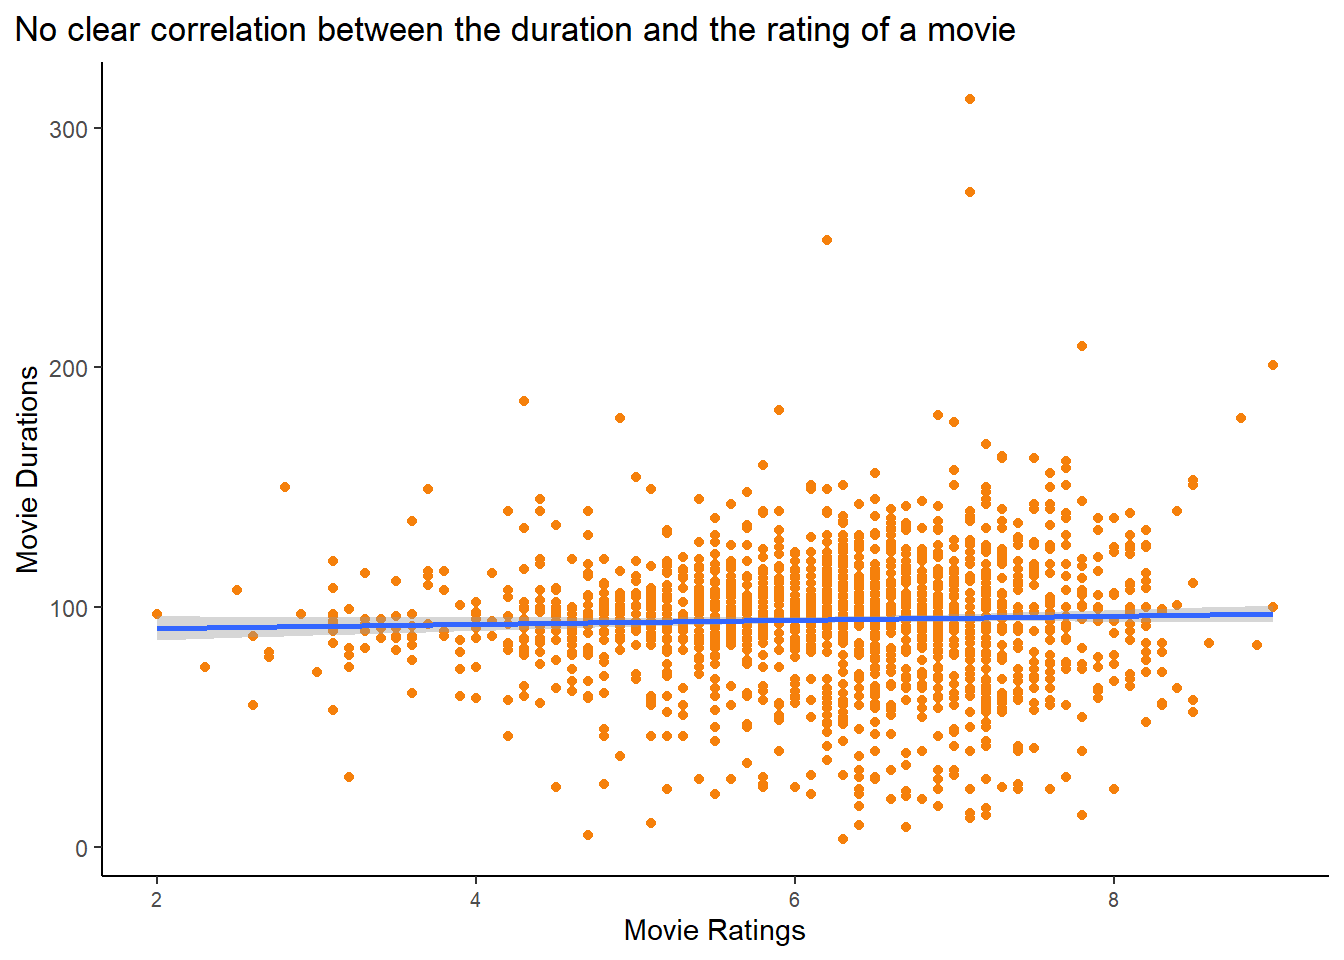
\includegraphics{Final_Project_files/figure-latex/unnamed-chunk-16-1.pdf}

The visualization shows movies are added to Netflix all year round, and
there is a roughly even distribution of movies across all months.
Therefore, we can safely carry out our analysis when we compare holiday
seasons to non-holiday seasons.

Now we are done with checking the basis of our analysis, we want to gain
more information from the data set to have a better understanding of it.
One thing really triggered our interests is the relationship between
ratings and the lengths of the movies.

\begin{Shaded}
\begin{Highlighting}[]
\FunctionTok{ggplot}\NormalTok{(merged, }\FunctionTok{aes}\NormalTok{(}\AttributeTok{x =}\NormalTok{ rating, }\AttributeTok{y =}\NormalTok{ duration)) }\SpecialCharTok{+}
  \FunctionTok{geom\_point}\NormalTok{(}\AttributeTok{color =} \StringTok{"\#F5800B"}\NormalTok{) }\SpecialCharTok{+}
  \FunctionTok{geom\_smooth}\NormalTok{(}\AttributeTok{method =} \StringTok{"lm"}\NormalTok{)}\SpecialCharTok{+}
  \FunctionTok{labs}\NormalTok{(}\AttributeTok{x =} \StringTok{"Movie Ratings"}\NormalTok{,}
       \AttributeTok{y =} \StringTok{"Movie Durations"}\NormalTok{,}
       \AttributeTok{title =} \StringTok{"No clear correlation between the duration and the rating of a movie"}\NormalTok{) }\SpecialCharTok{+}
  \FunctionTok{theme\_classic}\NormalTok{() }\SpecialCharTok{+}
  \FunctionTok{theme}\NormalTok{(}\AttributeTok{plot.title.position =} \StringTok{"plot"}\NormalTok{,}
        \AttributeTok{axis.text.x =} \FunctionTok{element\_text}\NormalTok{(}\AttributeTok{size =} \FloatTok{7.5}\NormalTok{),}
        \AttributeTok{legend.position =} \StringTok{"none"}\NormalTok{)}
\end{Highlighting}
\end{Shaded}

\begin{verbatim}
## `geom_smooth()` using formula = 'y ~ x'
\end{verbatim}

\begin{verbatim}
## Warning: Removed 21 rows containing non-finite values (`stat_smooth()`).
\end{verbatim}

\begin{verbatim}
## Warning: Removed 21 rows containing missing values (`geom_point()`).
\end{verbatim}

\includegraphics{Final_Project_files/figure-latex/unnamed-chunk-17-1.pdf}

However, although we anticipated that the ratings of movies that are
either too long or too short may receive low ratings, we cannot actually
get this conclusion from the plot. There seems to be no correlation
between the duration and the rating of a movie just through observing
the plot.

We are also curious about the what movie genres are included in the
dataset.

\begin{Shaded}
\begin{Highlighting}[]
\NormalTok{merged }\SpecialCharTok{|\textgreater{}}
  \FunctionTok{filter}\NormalTok{(release\_year }\SpecialCharTok{\textgreater{}=} \DecValTok{2010}\NormalTok{) }\SpecialCharTok{|\textgreater{}}
  \FunctionTok{separate\_rows}\NormalTok{(listed\_in, }\AttributeTok{sep =} \StringTok{", "}\NormalTok{) }\SpecialCharTok{|\textgreater{}} 
  \FunctionTok{group\_by}\NormalTok{(listed\_in) }\SpecialCharTok{|\textgreater{}} 
  \FunctionTok{summarise}\NormalTok{(}\AttributeTok{count =} \FunctionTok{n}\NormalTok{()) }\SpecialCharTok{|\textgreater{}}
  \FunctionTok{arrange}\NormalTok{(}\FunctionTok{desc}\NormalTok{(count))}
\end{Highlighting}
\end{Shaded}

\begin{verbatim}
## # A tibble: 20 x 2
##    listed_in                count
##    <chr>                    <int>
##  1 International Movies       738
##  2 Dramas                     636
##  3 Comedies                   383
##  4 Documentaries              280
##  5 Independent Movies         234
##  6 Thrillers                  209
##  7 Stand-Up Comedy            204
##  8 Action & Adventure         182
##  9 Children & Family Movies   156
## 10 Romantic Movies            143
## 11 Horror Movies              106
## 12 Music & Musicals            81
## 13 Sports Movies               63
## 14 LGBTQ Movies                41
## 15 Sci-Fi & Fantasy            37
## 16 Anime Features              15
## 17 Cult Movies                 14
## 18 Faith & Spirituality        13
## 19 Movies                       4
## 20 Classic Movies               1
\end{verbatim}

\hypertarget{movies-count-by-genre}{%
\paragraph{Movies count by genre}\label{movies-count-by-genre}}

\begin{Shaded}
\begin{Highlighting}[]
\CommentTok{\#create a tibble in longer format with rows for each combination of movie name and movie type from 2010 to 2013}
\NormalTok{merged\_long\_10\_13 }\OtherTok{\textless{}{-}}\NormalTok{ merged }\SpecialCharTok{|\textgreater{}}
  \FunctionTok{filter}\NormalTok{(release\_year }\SpecialCharTok{\textgreater{}=} \DecValTok{2010}\NormalTok{) }\SpecialCharTok{|\textgreater{}}
  \FunctionTok{filter}\NormalTok{(release\_year }\SpecialCharTok{\textless{}} \DecValTok{2014}\NormalTok{) }\SpecialCharTok{|\textgreater{}}
  \FunctionTok{separate\_rows}\NormalTok{(listed\_in, }\AttributeTok{sep =} \StringTok{", "}\NormalTok{) }\SpecialCharTok{|\textgreater{}} 
  \FunctionTok{group\_by}\NormalTok{(release\_year,listed\_in) }\SpecialCharTok{|\textgreater{}} 
  \FunctionTok{summarise}\NormalTok{(}\AttributeTok{count =} \FunctionTok{n}\NormalTok{())}

\CommentTok{\#create a tibble in longer format with rows for each combination of movie name and movie type from 2014 to 2017}
\NormalTok{merged\_long\_14\_17 }\OtherTok{\textless{}{-}}\NormalTok{ merged }\SpecialCharTok{|\textgreater{}}
  \FunctionTok{filter}\NormalTok{(release\_year }\SpecialCharTok{\textgreater{}=} \DecValTok{2014}\NormalTok{) }\SpecialCharTok{|\textgreater{}}
  \FunctionTok{filter}\NormalTok{(release\_year }\SpecialCharTok{\textless{}} \DecValTok{2018}\NormalTok{) }\SpecialCharTok{|\textgreater{}}
  \FunctionTok{separate\_rows}\NormalTok{(listed\_in, }\AttributeTok{sep =} \StringTok{", "}\NormalTok{) }\SpecialCharTok{|\textgreater{}} 
  \FunctionTok{group\_by}\NormalTok{(release\_year,listed\_in) }\SpecialCharTok{|\textgreater{}} 
  \FunctionTok{summarise}\NormalTok{(}\AttributeTok{count =} \FunctionTok{n}\NormalTok{())}

\CommentTok{\#create a tibble in longer format with rows for each combination of movie name and movie type from 2018 to 2021}
\NormalTok{merged\_long\_18\_21 }\OtherTok{\textless{}{-}}\NormalTok{ merged }\SpecialCharTok{|\textgreater{}}
  \FunctionTok{filter}\NormalTok{(release\_year }\SpecialCharTok{\textgreater{}=} \DecValTok{2018}\NormalTok{) }\SpecialCharTok{|\textgreater{}}
  \FunctionTok{filter}\NormalTok{(release\_year }\SpecialCharTok{\textless{}} \DecValTok{2022}\NormalTok{) }\SpecialCharTok{|\textgreater{}}
  \FunctionTok{separate\_rows}\NormalTok{(listed\_in, }\AttributeTok{sep =} \StringTok{", "}\NormalTok{) }\SpecialCharTok{|\textgreater{}} 
  \FunctionTok{group\_by}\NormalTok{(release\_year,listed\_in) }\SpecialCharTok{|\textgreater{}} 
  \FunctionTok{summarise}\NormalTok{(}\AttributeTok{count =} \FunctionTok{n}\NormalTok{())}
\end{Highlighting}
\end{Shaded}

Overall, there are an increasing number of movies produced each year
from 2010 to 2021, following the previous observation. Further, we see
that ``International Movies'', ``Dramas'', and ``Comedies'' appear the
most frequently. We wanted to see if this still holds true in each year
since 2010, so we will check the distribution of movie genres across
different years. Since there are many years in the data, we are going to
take a look at the distributions of the movie genres in three plots,
from year 2010 to 2013, 2014 to 2017, and 2018 to 2021 respectively.

\begin{Shaded}
\begin{Highlighting}[]
\CommentTok{\# Create distribution plot for year 2010{-}2013}
\FunctionTok{ggplot}\NormalTok{(merged\_long\_10\_13, }\FunctionTok{aes}\NormalTok{(}\AttributeTok{x =}\NormalTok{ release\_year, }\AttributeTok{y =}\NormalTok{ count, }\AttributeTok{fill =} \FunctionTok{reorder}\NormalTok{(listed\_in, count))) }\SpecialCharTok{+} 
  \FunctionTok{geom\_bar}\NormalTok{(}\AttributeTok{stat =} \StringTok{"identity"}\NormalTok{,}
           \AttributeTok{position =} \StringTok{"dodge"}\NormalTok{,}
           \AttributeTok{color =} \StringTok{"black"}\NormalTok{) }\SpecialCharTok{+} 
  \FunctionTok{scale\_fill\_viridis}\NormalTok{(}\AttributeTok{discrete =} \ConstantTok{TRUE}\NormalTok{) }\SpecialCharTok{+}
  \FunctionTok{labs}\NormalTok{(}\AttributeTok{x =} \StringTok{"Years"}\NormalTok{,}
       \AttributeTok{y =} \StringTok{"Count of each movie genre"}\NormalTok{,}
       \AttributeTok{title =} \StringTok{"The distributions of movie genres across years"}\NormalTok{,}
       \AttributeTok{subtitle =} \StringTok{"From 2010 to 2013"}\NormalTok{) }\SpecialCharTok{+}
  \FunctionTok{theme\_classic}\NormalTok{() }\SpecialCharTok{+}
  \FunctionTok{theme}\NormalTok{(}\AttributeTok{plot.margin =} \FunctionTok{unit}\NormalTok{(}\FunctionTok{c}\NormalTok{(}\DecValTok{0}\NormalTok{, }\DecValTok{0}\NormalTok{, }\DecValTok{0}\NormalTok{, }\DecValTok{0}\NormalTok{), }\StringTok{"cm"}\NormalTok{),}
        \AttributeTok{plot.title.position =} \StringTok{"plot"}\NormalTok{) }\SpecialCharTok{+}
  \FunctionTok{guides}\NormalTok{(}\AttributeTok{fill =} \FunctionTok{guide\_legend}\NormalTok{(}\StringTok{"Movie Genres"}\NormalTok{))}
\end{Highlighting}
\end{Shaded}

\includegraphics{Final_Project_files/figure-latex/unnamed-chunk-20-1.pdf}

\begin{Shaded}
\begin{Highlighting}[]
\CommentTok{\#create distribution plot for year 2014{-}2017}
\FunctionTok{ggplot}\NormalTok{(merged\_long\_14\_17, }\FunctionTok{aes}\NormalTok{(}\AttributeTok{x =}\NormalTok{ release\_year, }\AttributeTok{y =}\NormalTok{ count, }\AttributeTok{fill =} \FunctionTok{reorder}\NormalTok{(listed\_in, count))) }\SpecialCharTok{+} 
  \FunctionTok{geom\_bar}\NormalTok{(}\AttributeTok{stat =} \StringTok{"identity"}\NormalTok{,}
           \AttributeTok{position =} \StringTok{"dodge"}\NormalTok{,}
           \AttributeTok{color =} \StringTok{"black"}\NormalTok{) }\SpecialCharTok{+} 
  \FunctionTok{scale\_fill\_viridis}\NormalTok{(}\AttributeTok{discrete =} \ConstantTok{TRUE}\NormalTok{) }\SpecialCharTok{+}
  \FunctionTok{labs}\NormalTok{(}\AttributeTok{x =} \StringTok{"Years"}\NormalTok{,}
       \AttributeTok{y =} \StringTok{"Count of each movie genre"}\NormalTok{,}
       \AttributeTok{title =} \StringTok{"The distributions of movie genres across years"}\NormalTok{,}
       \AttributeTok{subtile =} \StringTok{"From 2014 to 2017"}\NormalTok{) }\SpecialCharTok{+}
  \FunctionTok{theme\_classic}\NormalTok{() }\SpecialCharTok{+}
  \FunctionTok{theme}\NormalTok{(}\AttributeTok{plot.margin =} \FunctionTok{unit}\NormalTok{(}\FunctionTok{c}\NormalTok{(}\DecValTok{0}\NormalTok{, }\DecValTok{0}\NormalTok{, }\DecValTok{0}\NormalTok{, }\DecValTok{0}\NormalTok{), }\StringTok{"cm"}\NormalTok{),}
        \AttributeTok{plot.title.position =} \StringTok{"plot"}\NormalTok{) }\SpecialCharTok{+}
  \FunctionTok{guides}\NormalTok{(}\AttributeTok{fill =} \FunctionTok{guide\_legend}\NormalTok{(}\StringTok{"Movie Genres"}\NormalTok{))}
\end{Highlighting}
\end{Shaded}

\includegraphics{Final_Project_files/figure-latex/unnamed-chunk-21-1.pdf}

\begin{Shaded}
\begin{Highlighting}[]
\CommentTok{\#create distribution plot for year 2018{-}2021}
\FunctionTok{ggplot}\NormalTok{(merged\_long\_18\_21, }\FunctionTok{aes}\NormalTok{(}\AttributeTok{x =}\NormalTok{ release\_year, }\AttributeTok{y =}\NormalTok{ count, }\AttributeTok{fill =} \FunctionTok{reorder}\NormalTok{(listed\_in, count))) }\SpecialCharTok{+} 
  \FunctionTok{geom\_bar}\NormalTok{(}\AttributeTok{stat =} \StringTok{"identity"}\NormalTok{,}
           \AttributeTok{position =} \StringTok{"dodge"}\NormalTok{,}
           \AttributeTok{color =} \StringTok{"black"}\NormalTok{) }\SpecialCharTok{+} 
  \FunctionTok{scale\_fill\_viridis}\NormalTok{(}\AttributeTok{discrete =} \ConstantTok{TRUE}\NormalTok{) }\SpecialCharTok{+}
  \FunctionTok{labs}\NormalTok{(}\AttributeTok{x =} \StringTok{"Years"}\NormalTok{,}
       \AttributeTok{y =} \StringTok{"Count of each movie genre"}\NormalTok{,}
       \AttributeTok{title =} \StringTok{"The distributions of movie genres across years"}\NormalTok{,}
       \AttributeTok{subtitle =} \StringTok{"From 2018 to 2021"}\NormalTok{) }\SpecialCharTok{+}
  \FunctionTok{theme\_classic}\NormalTok{() }\SpecialCharTok{+}
  \FunctionTok{theme}\NormalTok{(}\AttributeTok{plot.margin =} \FunctionTok{unit}\NormalTok{(}\FunctionTok{c}\NormalTok{(}\DecValTok{0}\NormalTok{, }\DecValTok{0}\NormalTok{, }\DecValTok{0}\NormalTok{, }\DecValTok{0}\NormalTok{), }\StringTok{"cm"}\NormalTok{),}
        \AttributeTok{plot.title.position =} \StringTok{"plot"}\NormalTok{) }\SpecialCharTok{+}
  \FunctionTok{guides}\NormalTok{(}\AttributeTok{fill =} \FunctionTok{guide\_legend}\NormalTok{(}\StringTok{"Movie Genres"}\NormalTok{))}
\end{Highlighting}
\end{Shaded}

\includegraphics{Final_Project_files/figure-latex/unnamed-chunk-22-1.pdf}

From the plots we can clearly observe that ``International Movies'',
``Dramas'', and ``Comedies'' appeared the most often in most of the
years from 2010 to 2021. Can this possibly indicate any trends about the
public's movie tastes? Further researches are needed to gain more
insights.

We found that the majority of the movies has several genres attached to
it, so we wanted to simplify the genres to include only one category.

\begin{Shaded}
\begin{Highlighting}[]
\NormalTok{merged }\OtherTok{\textless{}{-}}\NormalTok{ merged }\SpecialCharTok{|\textgreater{}}
  \FunctionTok{mutate}\NormalTok{(}\AttributeTok{genre =} \FunctionTok{case\_when}\NormalTok{(}
    \FunctionTok{grepl}\NormalTok{(}\StringTok{"Dramas"}\NormalTok{, listed\_in) }\SpecialCharTok{\textasciitilde{}} \StringTok{"Dramas"}\NormalTok{,}
    \FunctionTok{grepl}\NormalTok{(}\StringTok{"Comedies"}\NormalTok{, listed\_in) }\SpecialCharTok{\textasciitilde{}} \StringTok{"Comedies"}\NormalTok{,}
    \FunctionTok{grepl}\NormalTok{(}\StringTok{"Comedy"}\NormalTok{, listed\_in) }\SpecialCharTok{\textasciitilde{}} \StringTok{"Comedies"}\NormalTok{,}
    \FunctionTok{grepl}\NormalTok{(}\StringTok{"Documentaries"}\NormalTok{, listed\_in) }\SpecialCharTok{\textasciitilde{}} \StringTok{"Documentaries"}\NormalTok{,}
    \FunctionTok{grepl}\NormalTok{(}\StringTok{"Thrillers"}\NormalTok{, listed\_in) }\SpecialCharTok{\textasciitilde{}} \StringTok{"Thrillers"}\NormalTok{,}
    \FunctionTok{grepl}\NormalTok{(}\StringTok{"Action"}\NormalTok{, listed\_in) }\SpecialCharTok{\textasciitilde{}} \StringTok{"Action"}\NormalTok{,}
    \FunctionTok{grepl}\NormalTok{(}\StringTok{"Children"}\NormalTok{, listed\_in) }\SpecialCharTok{\textasciitilde{}} \StringTok{"Children"}\NormalTok{,}
    \FunctionTok{grepl}\NormalTok{(}\StringTok{"Romantic"}\NormalTok{, listed\_in) }\SpecialCharTok{\textasciitilde{}} \StringTok{"Romantic"}\NormalTok{,}
    \FunctionTok{grepl}\NormalTok{(}\StringTok{"Horror Movies"}\NormalTok{, listed\_in) }\SpecialCharTok{\textasciitilde{}} \StringTok{"Thrillers"}\NormalTok{,}
    \FunctionTok{grepl}\NormalTok{(}\StringTok{"Music"}\NormalTok{, listed\_in) }\SpecialCharTok{\textasciitilde{}} \StringTok{"Music"}\NormalTok{,}
    \ConstantTok{TRUE} \SpecialCharTok{\textasciitilde{}} \ConstantTok{NA}\NormalTok{))}

\NormalTok{merged }\SpecialCharTok{|\textgreater{}}
  \FunctionTok{filter}\NormalTok{(release\_year }\SpecialCharTok{\textgreater{}=} \DecValTok{2010}\NormalTok{) }\SpecialCharTok{|\textgreater{}}
  \FunctionTok{group\_by}\NormalTok{(genre) }\SpecialCharTok{|\textgreater{}}
  \FunctionTok{summarise}\NormalTok{(}\AttributeTok{count =} \FunctionTok{n}\NormalTok{()) }\SpecialCharTok{|\textgreater{}}
  \FunctionTok{arrange}\NormalTok{(}\FunctionTok{desc}\NormalTok{(count))}
\end{Highlighting}
\end{Shaded}

\begin{verbatim}
## # A tibble: 9 x 2
##   genre         count
##   <chr>         <int>
## 1 Dramas          636
## 2 Comedies        466
## 3 Documentaries   277
## 4 Thrillers       155
## 5 Action          108
## 6 Children         46
## 7 <NA>              7
## 8 Music             6
## 9 Romantic          5
\end{verbatim}

After simplifying, we see that ``Dramas'', ``Comedies'', and
``Documentaries'' are now the most-frequently appeared genres since
2010.

\begin{Shaded}
\begin{Highlighting}[]
\NormalTok{merged }\SpecialCharTok{|\textgreater{}}
  \FunctionTok{ggplot}\NormalTok{(}\FunctionTok{aes}\NormalTok{(}\AttributeTok{x =}\NormalTok{ rating, }\AttributeTok{y =} \FunctionTok{as.factor}\NormalTok{(genre), }\AttributeTok{fill =} \FunctionTok{as.factor}\NormalTok{(genre), }\AttributeTok{alpha =} \DecValTok{1}\NormalTok{)) }\SpecialCharTok{+}
  \FunctionTok{geom\_density\_ridges}\NormalTok{() }\SpecialCharTok{+}
  \FunctionTok{labs}\NormalTok{(}\AttributeTok{title =} \StringTok{"User ratings on IMDb in different genres"}\NormalTok{,}
       \AttributeTok{subtitle =} \StringTok{"The distributions of ratings are different in different genres"}\NormalTok{,}
       \AttributeTok{x =} \StringTok{"User Rating"}\NormalTok{,}
       \AttributeTok{y =} \StringTok{"Movie Genre"}\NormalTok{) }\SpecialCharTok{+} 
   \FunctionTok{scale\_fill\_manual}\NormalTok{(}\AttributeTok{values =} \FunctionTok{c}\NormalTok{(}\StringTok{"\#EBE224"}\NormalTok{,}\StringTok{"\#006EDD"}\NormalTok{,}\StringTok{"\#5ED389"}\NormalTok{,}\StringTok{"\#6E4400"}\NormalTok{,}
                                \StringTok{"\#8908E2"}\NormalTok{,}\StringTok{"\#FF8747"}\NormalTok{,}\StringTok{"\#FF6CE0"}\NormalTok{,}\StringTok{"\#FF0000"}\NormalTok{,}
                                \StringTok{"\#D09452"}\NormalTok{)) }\SpecialCharTok{+} 
  \FunctionTok{theme}\NormalTok{(}\AttributeTok{legend.position =} \StringTok{"none"}\NormalTok{,}
        \AttributeTok{plot.title.position =} \StringTok{"plot"}\NormalTok{,}
        \AttributeTok{panel.grid.major.x =} \FunctionTok{element\_blank}\NormalTok{(),}
        \AttributeTok{panel.grid.minor.x =} \FunctionTok{element\_blank}\NormalTok{(),}
        \AttributeTok{panel.grid.major.y =} \FunctionTok{element\_blank}\NormalTok{(),}
        \AttributeTok{panel.grid.minor.y =} \FunctionTok{element\_blank}\NormalTok{(),}
        \AttributeTok{panel.background =} \FunctionTok{element\_blank}\NormalTok{())}
\end{Highlighting}
\end{Shaded}

\begin{verbatim}
## Picking joint bandwidth of 0.355
\end{verbatim}

\begin{verbatim}
## Warning: Removed 20 rows containing non-finite values
## (`stat_density_ridges()`).
\end{verbatim}

\includegraphics{Final_Project_files/figure-latex/unnamed-chunk-24-1.pdf}

The plot shows different rating distributions across different movie
genres. For example, musical movies seem to receive high ratings, while
thrillers tend to receive low ratings. We will further explore this
trend in the following Question 2.

\hypertarget{data-analysis}{%
\subsubsection{Data Analysis}\label{data-analysis}}

\hypertarget{question-1-do-people-rate-movies-differently-over-the-years-since-2010}{%
\paragraph{Question 1: Do people rate movies differently over the years
since
2010?}\label{question-1-do-people-rate-movies-differently-over-the-years-since-2010}}

To find out if people give higher ratings over the years since 2010,
let's take a look from the plot first to see if there is any clear
trend.

\begin{Shaded}
\begin{Highlighting}[]
\NormalTok{merged }\SpecialCharTok{|\textgreater{}}
  \FunctionTok{filter}\NormalTok{(release\_year }\SpecialCharTok{\textgreater{}=} \DecValTok{2010}\NormalTok{) }\SpecialCharTok{|\textgreater{}}
  \FunctionTok{ggplot}\NormalTok{(}\FunctionTok{aes}\NormalTok{(}\AttributeTok{x =}\NormalTok{ release\_year, }\AttributeTok{y =}\NormalTok{ rating)) }\SpecialCharTok{+}
  \FunctionTok{geom\_jitter}\NormalTok{(}\AttributeTok{color =} \StringTok{"\#F5800B"}\NormalTok{) }\SpecialCharTok{+}
  \FunctionTok{geom\_smooth}\NormalTok{(}\AttributeTok{method =} \StringTok{"lm"}\NormalTok{) }\SpecialCharTok{+}
  \FunctionTok{labs}\NormalTok{(}\AttributeTok{x =} \StringTok{"Year released"}\NormalTok{,}
       \AttributeTok{y =} \StringTok{"Movie ratings"}\NormalTok{,}
       \AttributeTok{title =} \StringTok{"More recent movies received slightly lower ratings"}\NormalTok{) }\SpecialCharTok{+}
  \FunctionTok{scale\_x\_continuous}\NormalTok{(}\AttributeTok{breaks =} \FunctionTok{seq}\NormalTok{(}\DecValTok{2010}\NormalTok{, }\DecValTok{2021}\NormalTok{)) }\SpecialCharTok{+}
  \FunctionTok{theme}\NormalTok{(}\AttributeTok{plot.title.position =} \StringTok{"plot"}\NormalTok{) }\SpecialCharTok{+}
  \FunctionTok{theme\_classic}\NormalTok{(}\AttributeTok{base\_size =} \DecValTok{15}\NormalTok{)}
\end{Highlighting}
\end{Shaded}

\begin{verbatim}
## `geom_smooth()` using formula = 'y ~ x'
\end{verbatim}

\begin{verbatim}
## Warning: Removed 18 rows containing non-finite values (`stat_smooth()`).
\end{verbatim}

\begin{verbatim}
## Warning: Removed 18 rows containing missing values (`geom_point()`).
\end{verbatim}

\includegraphics{Final_Project_files/figure-latex/unnamed-chunk-25-1.pdf}

We see that movies released more recently tend to receive slightly lower
ratings than movies released earlier. This might be caused by a change
in the public taste of movies, but we are not sure about the exact
reasons behind this. In addition, as the plot shows, the amount of data
before 2015 is significantly less than the amount of data after 2015, so
the decreasing trend we found might not be accurate. To obtain more
accurate findings, we will build a model to see if such a decreasing
trend exists.

\begin{Shaded}
\begin{Highlighting}[]
\CommentTok{\# create a data frame that contains data since 2010}
\NormalTok{recent }\OtherTok{\textless{}{-}}\NormalTok{ merged }\SpecialCharTok{|\textgreater{}}
  \FunctionTok{filter}\NormalTok{(release\_year }\SpecialCharTok{\textgreater{}=} \DecValTok{2010}\NormalTok{)}

\CommentTok{\# convert release year to factors}
\NormalTok{recent}\SpecialCharTok{$}\NormalTok{release\_year }\OtherTok{\textless{}{-}} \FunctionTok{factor}\NormalTok{(recent}\SpecialCharTok{$}\NormalTok{release\_year)}

\CommentTok{\# fit a linear model with release year}
\NormalTok{mod\_yr }\OtherTok{\textless{}{-}} \FunctionTok{linear\_reg}\NormalTok{() }\SpecialCharTok{|\textgreater{}}
  \FunctionTok{set\_engine}\NormalTok{(}\StringTok{"lm"}\NormalTok{) }\SpecialCharTok{|\textgreater{}}
  \FunctionTok{fit}\NormalTok{(rating }\SpecialCharTok{\textasciitilde{}}\NormalTok{ release\_year, }\AttributeTok{data =}\NormalTok{ recent)}

\NormalTok{mod\_yr }\SpecialCharTok{|\textgreater{}}
  \FunctionTok{tidy}\NormalTok{()}
\end{Highlighting}
\end{Shaded}

\begin{verbatim}
## # A tibble: 12 x 5
##    term             estimate std.error statistic  p.value
##    <chr>               <dbl>     <dbl>     <dbl>    <dbl>
##  1 (Intercept)         5.47      0.248     22.1  5.60e-95
##  2 release_year2011    1.16      0.355      3.28 1.06e- 3
##  3 release_year2012    1.08      0.332      3.25 1.18e- 3
##  4 release_year2013    1.38      0.295      4.68 3.10e- 6
##  5 release_year2014    0.873     0.300      2.91 3.63e- 3
##  6 release_year2015    0.937     0.273      3.43 6.17e- 4
##  7 release_year2016    0.696     0.260      2.67 7.61e- 3
##  8 release_year2017    0.736     0.258      2.85 4.39e- 3
##  9 release_year2018    0.602     0.256      2.35 1.88e- 2
## 10 release_year2019    0.672     0.256      2.62 8.81e- 3
## 11 release_year2020    0.680     0.255      2.66 7.77e- 3
## 12 release_year2021    0.511     0.260      1.96 4.96e- 2
\end{verbatim}

\begin{Shaded}
\begin{Highlighting}[]
\CommentTok{\# check R\^{}2}
\FunctionTok{glance}\NormalTok{(mod\_yr)}
\end{Highlighting}
\end{Shaded}

\begin{verbatim}
## # A tibble: 1 x 12
##   r.squared adj.r.squared sigma statistic    p.value    df logLik   AIC   BIC
##       <dbl>         <dbl> <dbl>     <dbl>      <dbl> <dbl>  <dbl> <dbl> <dbl>
## 1    0.0267        0.0203  1.08      4.18 0.00000398    11 -2519. 5064. 5135.
## # i 3 more variables: deviance <dbl>, df.residual <int>, nobs <int>
\end{verbatim}

We can see from the model that, after 2010, where movies received an
average rating of 5.47, people are indeed giving lower ratings, as we
see the difference between each consecutive year and 2010 decreases,
although not significant. People tend to give around 6.63 in 2011 and
6.54 in 2012, but only tend to give 6.15 in 2020 and 5.98 in 2021.

To evaluate the strength of the fit of this model, we also checked the
\(R^2\) value, which turns out to be 0.027. Therefore, roughly only
2.7\% of the variability in movie ratings can be explained by their
release year. This suggests the year a movie is released might not be a
strong and appropriate predictor for its rating.

\hypertarget{question-2-do-movies-receive-lowerhigher-ratings-due-to-their-genres}{%
\paragraph{Question 2: Do movies receive lower/higher ratings due to
their
genres?}\label{question-2-do-movies-receive-lowerhigher-ratings-due-to-their-genres}}

To answer this question, we first create a linear model of rating and
genre.

\begin{Shaded}
\begin{Highlighting}[]
\CommentTok{\# fit a linear model}
\NormalTok{mod\_gr }\OtherTok{\textless{}{-}} \FunctionTok{linear\_reg}\NormalTok{() }\SpecialCharTok{|\textgreater{}}
  \FunctionTok{set\_engine}\NormalTok{(}\StringTok{"lm"}\NormalTok{) }\SpecialCharTok{|\textgreater{}}
  \FunctionTok{fit}\NormalTok{(rating }\SpecialCharTok{\textasciitilde{}}\NormalTok{ genre, }\AttributeTok{data =}\NormalTok{ recent)}

\NormalTok{mod\_gr }\SpecialCharTok{|\textgreater{}}
  \FunctionTok{tidy}\NormalTok{()}
\end{Highlighting}
\end{Shaded}

\begin{verbatim}
## # A tibble: 8 x 5
##   term               estimate std.error statistic  p.value
##   <chr>                 <dbl>     <dbl>     <dbl>    <dbl>
## 1 (Intercept)           5.91     0.0988    59.8   0       
## 2 genreChildren         0.215    0.180      1.20  2.32e- 1
## 3 genreComedies         0.104    0.110      0.946 3.44e- 1
## 4 genreDocumentaries    0.979    0.116      8.42  8.16e-17
## 5 genreDramas           0.260    0.107      2.44  1.48e- 2
## 6 genreMusic            1.67     0.427      3.92  9.30e- 5
## 7 genreRomantic         0.129    0.465      0.276 7.82e- 1
## 8 genreThrillers       -0.538    0.129     -4.18  3.09e- 5
\end{verbatim}

\begin{Shaded}
\begin{Highlighting}[]
\CommentTok{\# check R\^{}2}
\FunctionTok{glance}\NormalTok{(mod\_gr)}
\end{Highlighting}
\end{Shaded}

\begin{verbatim}
## # A tibble: 1 x 12
##   r.squared adj.r.squared sigma statistic  p.value    df logLik   AIC   BIC
##       <dbl>         <dbl> <dbl>     <dbl>    <dbl> <dbl>  <dbl> <dbl> <dbl>
## 1     0.134         0.131  1.02      37.1 1.68e-48     7 -2410. 4837. 4886.
## # i 3 more variables: deviance <dbl>, df.residual <int>, nobs <int>
\end{verbatim}

We see that after 2010 action movies, the baseline genre, receive an
average rating of 5.91. Musical movies receive an average rating of
7.58, which is the highest rating among all genres after 2010, while
thrillers only receive an average rating of 5.37, which is the lowest
rating among all genres after 2010. As for the most numerous movies in
the dataset, documentaries receive an average rating of 6.89, dramas
movies receive an average rating of 6.17, and comedies receive an
average rating of 6.01. It is somewhat expected that thrillers receive
low ratings, since most thrillers are of low quality.

The \(R^2\) of this model is 0.13. Therefore, roughly 13\% of the
variability in movie ratings can be explained by their genre. This
\(R^2\) value is greater than that of the year model, so the genre might
a better predictor for its rating than the year a movie is released in.

We also wanted to add genre to the model created in Question 1 to see
how it affects the rating.

\begin{Shaded}
\begin{Highlighting}[]
\NormalTok{mod\_full }\OtherTok{\textless{}{-}} \FunctionTok{linear\_reg}\NormalTok{() }\SpecialCharTok{|\textgreater{}}
  \FunctionTok{set\_engine}\NormalTok{(}\StringTok{"lm"}\NormalTok{) }\SpecialCharTok{|\textgreater{}}
  \FunctionTok{fit}\NormalTok{(rating }\SpecialCharTok{\textasciitilde{}}\NormalTok{ release\_year }\SpecialCharTok{+}\NormalTok{ genre, }\AttributeTok{data =}\NormalTok{ recent)}

\NormalTok{mod\_full }\SpecialCharTok{|\textgreater{}}
  \FunctionTok{tidy}\NormalTok{()}
\end{Highlighting}
\end{Shaded}

\begin{verbatim}
## # A tibble: 19 x 5
##    term               estimate std.error statistic  p.value
##    <chr>                 <dbl>     <dbl>     <dbl>    <dbl>
##  1 (Intercept)           5.41      0.248    21.9   2.43e-93
##  2 release_year2011      0.926     0.332     2.79  5.32e- 3
##  3 release_year2012      0.945     0.309     3.05  2.30e- 3
##  4 release_year2013      1.21      0.277     4.38  1.29e- 5
##  5 release_year2014      0.545     0.281     1.94  5.23e- 2
##  6 release_year2015      0.593     0.256     2.31  2.08e- 2
##  7 release_year2016      0.366     0.244     1.50  1.34e- 1
##  8 release_year2017      0.456     0.242     1.89  5.95e- 2
##  9 release_year2018      0.345     0.240     1.44  1.50e- 1
## 10 release_year2019      0.356     0.241     1.48  1.39e- 1
## 11 release_year2020      0.374     0.240     1.56  1.19e- 1
## 12 release_year2021      0.227     0.244     0.928 3.54e- 1
## 13 genreChildren         0.349     0.180     1.94  5.23e- 2
## 14 genreComedies         0.188     0.110     1.71  8.74e- 2
## 15 genreDocumentaries    1.07      0.117     9.19  1.14e-19
## 16 genreDramas           0.356     0.107     3.31  9.53e- 4
## 17 genreMusic            1.79      0.423     4.24  2.35e- 5
## 18 genreRomantic         0.317     0.462     0.686 4.93e- 1
## 19 genreThrillers       -0.437     0.129    -3.39  7.13e- 4
\end{verbatim}

\begin{Shaded}
\begin{Highlighting}[]
\CommentTok{\# check R\^{}2}
\FunctionTok{glance}\NormalTok{(mod\_full)}
\end{Highlighting}
\end{Shaded}

\begin{verbatim}
## # A tibble: 1 x 12
##   r.squared adj.r.squared sigma statistic  p.value    df logLik   AIC   BIC
##       <dbl>         <dbl> <dbl>     <dbl>    <dbl> <dbl>  <dbl> <dbl> <dbl>
## 1     0.162         0.153  1.00      17.9 4.14e-52    18 -2382. 4804. 4913.
## # i 3 more variables: deviance <dbl>, df.residual <int>, nobs <int>
\end{verbatim}

The model shows that, after 2010, when action movies received an average
rating of 5.42, people give lower ratings across the years. People tend
to give a rating of around 6.35 in 2011 and 6.36 in 2012, but only tend
to give a rating of 5.79 in 2020 and 5.65 in 2021. Again, we see the
same results that musicals receive an average rating of 7.21, which
makes it the highest-rated genre, while thrillers only receive an
average rating of 4.98, which makes it the lowest-rated genre. As for
the most numerous genres: dramas receive a rating of 5.77 on average,
comedies receive a rating of 5.61, and documentaries receive a rating of
6.49.

The adjusted \(R^2\) of this model is 0.15. Therefore, roughly 15\% of
the variability in movie ratings can be explained by their genre and
release year.

\hypertarget{question-3-does-a-movie-released-during-a-holiday-season-receive-a-higherlower-rating-than-a-movie-released-during-other-times-of-the-year}{%
\paragraph{Question 3: Does a movie released during a holiday season
receive a higher/lower rating than a movie released during other times
of the
year?}\label{question-3-does-a-movie-released-during-a-holiday-season-receive-a-higherlower-rating-than-a-movie-released-during-other-times-of-the-year}}

We start by calculating the average ratings of movies released during
the holiday season, non-holiday season, and all months.

We define the holiday season to be from Thanksgiving to Christmas, which
is from November to December.

\begin{Shaded}
\begin{Highlighting}[]
\NormalTok{recent }\SpecialCharTok{|\textgreater{}}
  \FunctionTok{filter}\NormalTok{(month }\SpecialCharTok{==} \DecValTok{11} \SpecialCharTok{|}\NormalTok{ month }\SpecialCharTok{==} \DecValTok{12}\NormalTok{) }\SpecialCharTok{|\textgreater{}}
  \FunctionTok{summarise}\NormalTok{(}\StringTok{\textasciigrave{}}\AttributeTok{mean rating}\StringTok{\textasciigrave{}} \OtherTok{=} \FunctionTok{mean}\NormalTok{(rating, }\AttributeTok{na.rm =} \ConstantTok{TRUE}\NormalTok{))}
\end{Highlighting}
\end{Shaded}

\begin{verbatim}
##   mean rating
## 1     6.18172
\end{verbatim}

The mean ratings of movies released in holiday seasons is 6.182.

\begin{Shaded}
\begin{Highlighting}[]
\NormalTok{recent }\SpecialCharTok{|\textgreater{}}
  \FunctionTok{filter}\NormalTok{(month }\SpecialCharTok{!=} \DecValTok{11} \SpecialCharTok{\&}\NormalTok{ month }\SpecialCharTok{!=} \DecValTok{12}\NormalTok{) }\SpecialCharTok{|\textgreater{}}
  \FunctionTok{summarise}\NormalTok{(}\StringTok{\textasciigrave{}}\AttributeTok{mean rating}\StringTok{\textasciigrave{}} \OtherTok{=} \FunctionTok{mean}\NormalTok{(rating, }\AttributeTok{na.rm =} \ConstantTok{TRUE}\NormalTok{))}
\end{Highlighting}
\end{Shaded}

\begin{verbatim}
##   mean rating
## 1    6.161604
\end{verbatim}

The mean ratings of movies released in non-holiday seasons is 6.162,
which is slightly lower than that of movies released during the holiday
season.

\begin{Shaded}
\begin{Highlighting}[]
\FunctionTok{mean}\NormalTok{(recent}\SpecialCharTok{$}\NormalTok{rating, }\AttributeTok{na.rm =} \ConstantTok{TRUE}\NormalTok{)}
\end{Highlighting}
\end{Shaded}

\begin{verbatim}
## [1] 6.164929
\end{verbatim}

The mean ratings of all movies is 6.165, which is also slightly lower
than that of movies released during the holiday season.

To summarize, the average rating is slightly higher for the movies
released during the holiday season, compared to movies released in
non-holiday seasons and all movies.

We also attempt to fit a linear model to further support our findings.

\begin{Shaded}
\begin{Highlighting}[]
\CommentTok{\# convert months to factors}
\NormalTok{recent}\SpecialCharTok{$}\NormalTok{month }\OtherTok{\textless{}{-}} \FunctionTok{factor}\NormalTok{(recent}\SpecialCharTok{$}\NormalTok{month)}

\CommentTok{\# create linear model}
\NormalTok{mod\_mth }\OtherTok{\textless{}{-}} \FunctionTok{linear\_reg}\NormalTok{() }\SpecialCharTok{|\textgreater{}}
  \FunctionTok{set\_engine}\NormalTok{(}\StringTok{"lm"}\NormalTok{) }\SpecialCharTok{|\textgreater{}}
  \FunctionTok{fit}\NormalTok{(rating }\SpecialCharTok{\textasciitilde{}}\NormalTok{ month, }\AttributeTok{data =}\NormalTok{ recent)}

\FunctionTok{tidy}\NormalTok{(mod\_mth)}
\end{Highlighting}
\end{Shaded}

\begin{verbatim}
## # A tibble: 12 x 5
##    term        estimate std.error statistic p.value
##    <chr>          <dbl>     <dbl>     <dbl>   <dbl>
##  1 (Intercept)   6.20       0.101    61.3    0     
##  2 month2        0.0370     0.141     0.263  0.792 
##  3 month3        0.0852     0.134     0.634  0.526 
##  4 month4       -0.204      0.137    -1.49   0.136 
##  5 month5       -0.0755     0.137    -0.551  0.582 
##  6 month6       -0.224      0.134    -1.68   0.0938
##  7 month7        0.0362     0.134     0.270  0.787 
##  8 month8       -0.154      0.139    -1.11   0.268 
##  9 month9       -0.0319     0.133    -0.239  0.811 
## 10 month10       0.142      0.136     1.05   0.295 
## 11 month11       0.0755     0.139     0.544  0.587 
## 12 month12      -0.103      0.135    -0.762  0.446
\end{verbatim}

\begin{Shaded}
\begin{Highlighting}[]
\CommentTok{\# check R\^{}2}
\FunctionTok{glance}\NormalTok{(mod\_mth)}
\end{Highlighting}
\end{Shaded}

\begin{verbatim}
## # A tibble: 1 x 12
##   r.squared adj.r.squared sigma statistic p.value    df logLik   AIC   BIC
##       <dbl>         <dbl> <dbl>     <dbl>   <dbl> <dbl>  <dbl> <dbl> <dbl>
## 1    0.0110       0.00453  1.09      1.70  0.0683    11 -2532. 5091. 5162.
## # i 3 more variables: deviance <dbl>, df.residual <int>, nobs <int>
\end{verbatim}

The table shows, for example, the average movie ratings in January is
6.2 and the average rating is 6.34 during October, while the average
movie rating in November is 6.28, and the average rating in December is
6.1. The adjusted \(R^2\) of this model is 0.011, which means roughly
only 1.1\% of the variability in movie ratings can be explained by their
release month.

This indicates movie ratings in November and December might not be
significantly different from other months in a year, but we cannot be
sure to draw this conclusion due to the weak model. Therefore, we will
conduct an ANOVA test below to check the difference. Our null hypothesis
is that there is no significant difference between the ratings for
movies released during holiday seasons and non-holiday seasons. We will
use the typical threshold of 0.05 for the alpha value.

\begin{Shaded}
\begin{Highlighting}[]
\CommentTok{\# create a column that discriminates between holiday and non{-}holiday seasons and convert it to factors}
\NormalTok{recent }\OtherTok{\textless{}{-}}\NormalTok{ recent }\SpecialCharTok{|\textgreater{}}
  \FunctionTok{mutate}\NormalTok{(}\AttributeTok{is\_nov\_dec =} \FunctionTok{ifelse}\NormalTok{(month }\SpecialCharTok{\%in\%} \FunctionTok{c}\NormalTok{(}\DecValTok{11}\NormalTok{, }\DecValTok{12}\NormalTok{), }\StringTok{"Nov\_Dec"}\NormalTok{, }\StringTok{"Other\_Months"}\NormalTok{),}
         \AttributeTok{is\_nov\_dec =} \FunctionTok{factor}\NormalTok{(is\_nov\_dec))}

\CommentTok{\# create an ANOVA model}
\NormalTok{anova\_model }\OtherTok{\textless{}{-}} \FunctionTok{aov}\NormalTok{(rating }\SpecialCharTok{\textasciitilde{}}\NormalTok{ is\_nov\_dec, }\AttributeTok{data =}\NormalTok{ recent)}

\FunctionTok{tidy}\NormalTok{(anova\_model)}
\end{Highlighting}
\end{Shaded}

\begin{verbatim}
## # A tibble: 2 x 6
##   term          df     sumsq meansq statistic p.value
##   <chr>      <dbl>     <dbl>  <dbl>     <dbl>   <dbl>
## 1 is_nov_dec     1    0.0942 0.0942    0.0791   0.779
## 2 Residuals   1686 2008.     1.19     NA       NA
\end{verbatim}

Since the p-value of 0.78 is larger than 0.05, we fail to reject the
null hypothesis. Consequently, there is not a difference between the
ratings for movies released during the holiday season and other months.

\hypertarget{results}{%
\subsubsection{Results}\label{results}}

\begin{itemize}
\tightlist
\item
  Q1
\end{itemize}

We found that people give slightly lower movies ratings over the years
since 2010. However, the trend might not be significant since the linear
model is weak.

Therefore, we propose that the lack of significance is hardly due to
shifts in user preferences or user behavior. In fact, the weak result
might be due to an increased number of movies produced over the years,
which caused more variation in ratings that is difficult to generalize.

\begin{itemize}
\tightlist
\item
  Q2
\end{itemize}

We found that movies of different genres indeed receive different
ratings. For example, musical movies receive an average rating of 7.58,
which is the highest-rated genre, while thrillers only receive an
average rating of 5.37, which is the lowest-rated genre.

The model combining release year and genre produced a stronger support
for our findings in Question 1 and Question 2.

This finding is particularly helpful as a user implication.
Specifically, when making decisions among cross-category movies, direct
comparison of numeric scores is less reliable or meaningful. Users
should consider other movies in the same genre in order to correctly
infer the reputation of said movies.

\begin{itemize}
\tightlist
\item
  Q3
\end{itemize}

As an extension to Q1, we looked at ratings while condtioning the
presence of major holidays. We found no significant difference between
ratings for movies released during the holiday season compared to other
months of the year from our linear model and ANOVA test.

\hypertarget{limitation}{%
\subsubsection{Limitation}\label{limitation}}

Several limitations should be considered in this study. The data used in
this project is highly skewed after 2015, which limits our ability to
gain insights into the trend across the entire timeline. Consequently,
the findings of this study may not be representative of the entire
population of movies. Our future steps could explore additional data
sources or use different sampling methods to mitigate this limitation.
Further, while this study explores several factors that contribute to
user ratings of movies, there could be unexplored factors that might
potentially be more predictive of these ratings. For example, sales data
and maturity rating could influence user ratings but were not included
in this analysis. Finally, due to the limitation of available data, we
were not able to confirm the submission time of the ratings. Instead, we
based our analysis on the release date of the movies. This may have
introduced some inaccuracies in our findings as user ratings may have
been submitted at different times after the movie was released.
Exploring alternative methods for estimating the timing of user ratings,
such as using data from social media or other online platforms, will
benefit the accuracy of the results.

\hypertarget{conclusion}{%
\subsection{Conclusion}\label{conclusion}}

In conclusion, our investigation into IMDb reviews and ratings has
revealed several key insights into the reliability and factors affecting
movie ratings. We found that there is a slight decline in movie ratings
over the years since 2010, suggesting that user preferences and
expectations might have shifted over time. Moreover, we discovered that
different genres of movies receive varying ratings, with musicals
enjoying the highest average rating and thrillers receiving the lowest.
However, we did not find a significant difference in ratings for movies
released during the holiday season compared to other months of the year.

These findings highlight the importance of taking a nuanced approach
when interpreting online movie reviews and ratings. Users should be
aware of the potential subjectivity and external factors that could
influence ratings and not solely rely on them for making decisions on
which movies to watch. By understanding the trends and variations in
user ratings, moviegoers can make more informed choices and find content
that best matches their preferences and interests. Ultimately, a deeper
understanding of online movie reviews and ratings can lead to better
decision-making processes for viewers and a more enjoyable
movie-watching experience.

\end{document}
